\documentclass{article}
\usepackage{ctex}
\usepackage{hyperref}
\usepackage{geometry}
\usepackage{amsmath}
\usepackage{caption}
\RequirePackage{longtable,multirow,array}
\RequirePackage{booktabs}
\usepackage{booktabs}
\usepackage{multicol}
\usepackage{longtable}
\usepackage{booktabs}
\usepackage{algorithm}
\usepackage{algpseudocode}
\usepackage{enumitem}
\usepackage[style=ieee,sorting=nyt]{biblatex}
\assignrefcontextentries[]{*}
\addbibresource{References.bib}
\geometry{left=1in, right=1in, top=1in, bottom=1in}
\hypersetup{hidelinks}
\hypersetup{bookmarksnumbered=true,
	bookmarksopen=true,
	colorlinks=true,
	linkcolor=black,
	citecolor=blue,
	urlcolor=black}
\usepackage{tikz}
\usepackage{pgfplotstable}
\usepackage{pgfplots}
\pgfplotsset{compat=1.18}
\captionsetup{justification=centering}
\captionsetup[figure]{name={Fig.},labelsep=space,labelfont=bf}
\captionsetup[table]{name={Table},labelsep=space,labelfont=bf}
\CTEXoptions[today=old, contentsname=Contents]
\newcommand{\authyear}[1]{\citeauthor{#1} (\citeyear{#1})}
\setmainfont{Arial}

\newcommand{\toB}[1]{\color{blue}#1\color{black}}

\begin{document}
	\title{\vspace{-2.25cm} Multimodal Abnormity-Aware Model\\for Ocular Disease Diagnosis}
	\author{Siqi Pan}
	\date{}
	\maketitle
	
	\section*{Abstract}
	
	TEXT: abstract
	
	\section{Background}
	Ocular diseases can be diagnosed through various methods, including using optical coherence tomography (OCT) and color fundus images. Ophthalmologists usually identify ocular abnormalities to deduce the disease. Traditionally, the diagnosis primarily depends on the professional experience and knowledge of the ophthalmologists, which may result in high misdiagnosis rate and under-utilization of medical data. With the widespread application of artificial intelligence (AI), deep learning (DL) has made great contributions in providing support to patients in remote areas by sharing expert knowledge \autocite{Ichhpujani_Thakur_2021}. By leveraging DL, researchers have developed auxiliary diagnosis programs to help ophthalmologists in the process. Many studies use convolutional neural network (CNN) to analyze ocular images. Some commonly used CNNs are VGG, ResNet, and Inception \autocite{daich2023artificial}. And for segmenting images and finding abnormalities, U-net is widely used \autocite{Ronneberger_Fischer_Brox_2015}. With regards to training CNNs, most studies use transferred learning, which consists of three steps: learning, fine-tuning, and validation.
	
	Some studies directly predict the disease from OCT images.
	\authyear{li2019deep} used ResNet to analyze OCT images and distinguish between choroidal neovascularization (CNV), diabetic macular edema (DME), drusen, and healthy eyes. In addition, they performed occlusion testing to find out the regions that are the most important in diagnosis \autocite{li2019deep}. 
	\authyear{yoo2021feasibility} used generative adversarial network (GAN) and Inception-v3 together with a few-shot dataset to investigate the feasibility of improving OCT diagnosis of rare ocular diseases \autocite{yoo2021feasibility}. They handled the issues of training image shortage and data imbalance by creating ocular disease OCT images from healthy OCT images. \authyear{Kermany2018} conducts medical diagnosis and identifies treatable diseases by image-based deep learning. They also provided a widely used database including more than one hundred thousand OCT labeled images for 3 diseases \autocite{Kermany2018}.
	
	Some other studies can identify ocular abnormalities from annotated OCT images.
	\authyear{camino2018deep} used DL to identify the region of preserved photoreceptors on \textit{en face} OCT in choroideremia and retinitis pigmentosa (RP) \autocite{camino2018deep}. 
	\authyear{srinivasan2014fully} detected DME and dry age-related macular degeneration (dry AMD) from OCT images by flattening the image and using support vector machine (SVM) to extract the thickness information of the retinal layers \autocite{srinivasan2014fully}. 
	\authyear{leandro2023oct} implemented VGG to identify up to 8 kinds of key abnormalities and hence detect multiple diseases by using central fovea cross-section OCT \autocite{leandro2023oct}. \authyear{Fang_Wang2019} developed a novel lesion-aware CNN, called LACNN, to simulate the ophthalmologists' diagnosis that focuses on ocular abnormalities. The LACNN is a U-net-like CNN which incorporates VGG16 as the baseline, and the result is impressive \autocite{Fang_Wang2019}.
	
	Other studies use fundus images to predict ocular diseases.
	\authyear{masumoto2019accuracy} trained deep CNN with ultrawide-field fundus images to make the CNN capable of diagnosing RP \autocite{masumoto2019accuracy}. 
	\authyear{chen2021artificial} uses color fundus photographs and multiple types of CNN (Inception V3, Inception Resnet V2, and Xception) to develop a method of early detection of RP \autocite{chen2021artificial}. 
	\authyear{li2022development} uses CNN to detect up to 12 fundus diseases based on colour fundus photography \autocite{li2022development}. \authyear{Son2023} presented a novel architectural and algorithmic design to comprehensively identify 15 abnormalities and diagnose 8 major ocular diseases from macula-centered fundus images. They defined a notion of counterfactual attribution ratio (CAR) to interpret the system's diagnostic reason and disclose the relationship between abnormalities and diseases \autocite{Son2023}.
	
	In recent years, more and more DL systems began to use multi-modal information to predict ocular diseases. For automated detection system, retrieving features from both OCT images and fundus images can effectively keep the diagnosis away from bias and incompleteness. It is not always necessary to yield a better automated diagnosis result, but it does help ophthalmologist to make more accurate and holistic clinical decisions. For instance, \authyear{liu2023prediction} combined OCT and fundus images to evaluate visual impairment in RP in terms of best-corrected visual acuity(BCVA) \autocite{liu2023prediction}. \authyear{Xu2021} leveraged a bi-modal CNN to diagnose AMD and polypoidal choroidal vasculopathy (PCV), where the architecture uses fundus and OCT images as input for transferred learning CNN and concatenates the retrieved features to classify 3 diseases including dry AMD, wet AMD and PCV \autocite{Xu2021}. And \author{Andrearczyk2018} ingeniously combined medical images and biomedical textual information to discriminate different diseases, which is a novel method for the usage of multi-modal application \autocite{Andrearczyk2018}.
	
	The key technical problem of multi-modal diagnosis is how to fuse the results from multifarious sources. There are three types of fusion, namely early, late, and hybrid fusion. Deciding on the optimal type of fusion is part of the exploratory process in the application of DL methods \autocite{Ichhpujani_Thakur_2021}.
	
	
	
	\section{Overview}
	
	We develop the Multimodal Abnormity-Aware Model (MAAM) to aid ophthalmologists in diagnosing ocular diseases. It considers both OCT and color fundus image inputs. In addition, it simulates the decision-making process of ophthalmologists when they examine patients, namely, first identifying the abnormities, and then deducing the disease. The model is designed in a way that partly opens up the ``black box'' of DL and presents more interpretable information to ophthalmologists for the reference. 
	
	\begin{figure}[htbp]
		\centering
		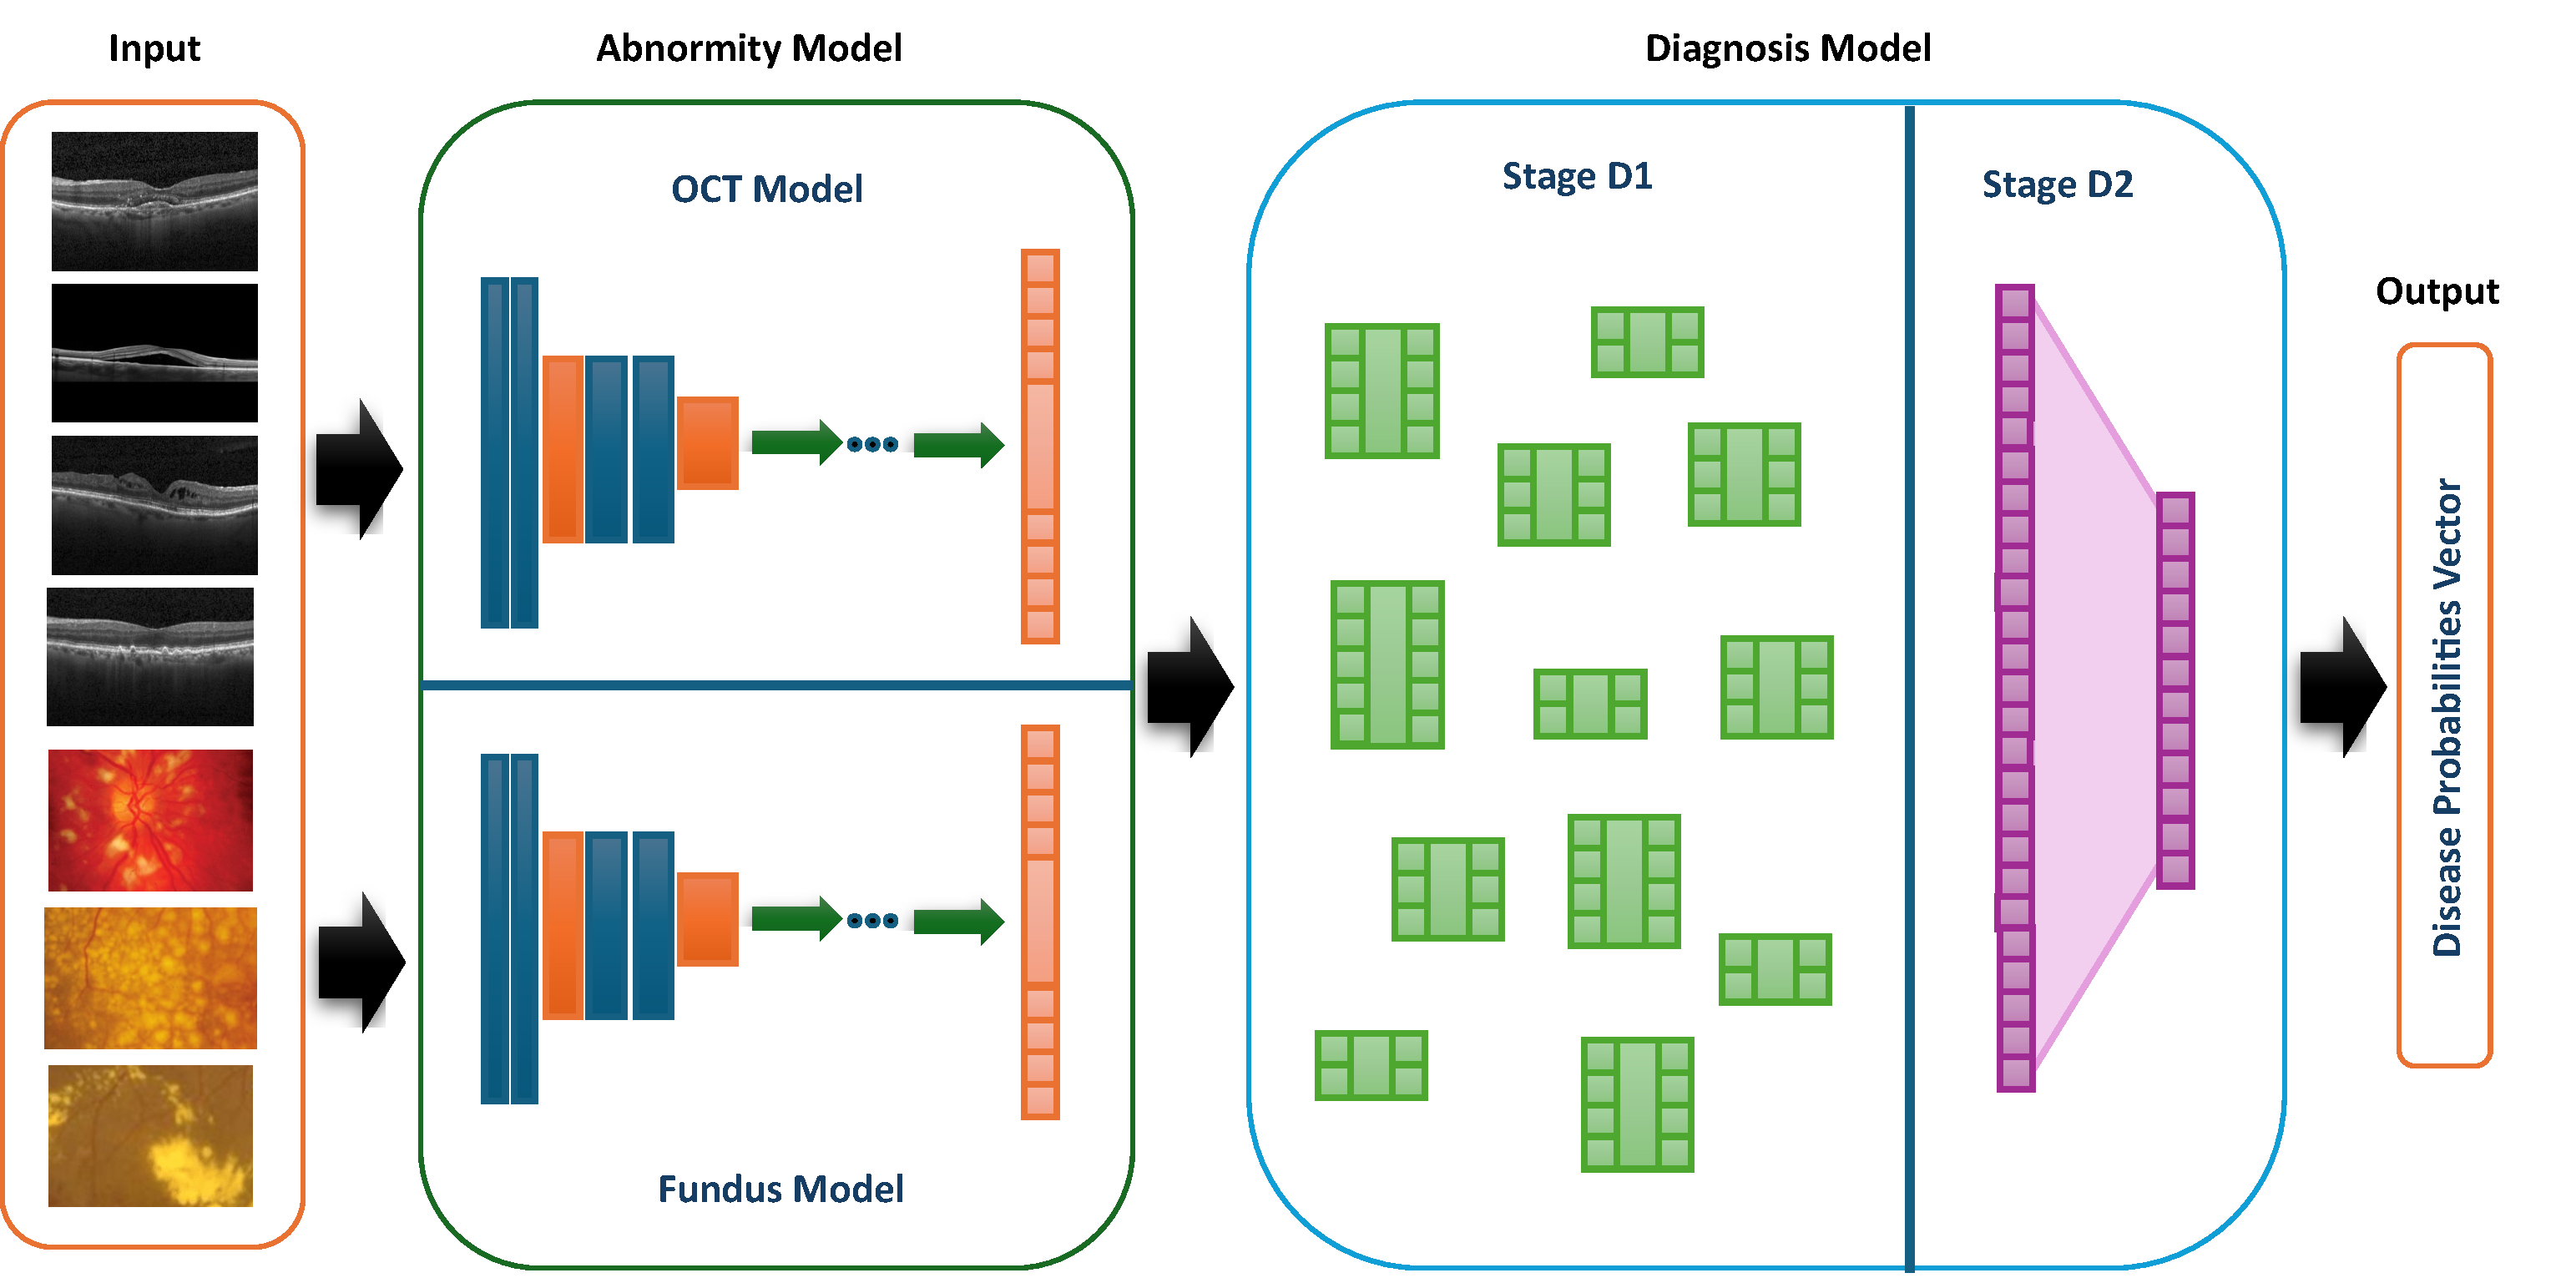
\includegraphics[width=\linewidth]{Figs/model_overview.pdf}
		\caption{Model Overview}
		\vspace{0.3cm}
		\label{fig:3_parts}
	\end{figure}
	
	The structure of the MAAM is shown in Fig.~\ref{fig:3_parts}. It consists of 2 submodels: the Abnormity Model and the Diagnosis Model. We input multiple OCT and fundus images to the Abnormity Models, and output the classification of abnormities as an input to the Diagnosis Model, which yields disease probabilities as the final result.
	
	\vspace{0.5cm}
	
	The Abnormity Models are de facto classifiers for abnormities, which are symptoms that can be directly observed in the images. The MAAM identifies 11 OCT abnormities and 8 Fundus abnormities, as shown in Fig.~\ref{fig:OCT_abnormities} and Fig.~\ref{fig:fundus_abnormities}. The abbreviations and detail information of abnormities and diseases are tabulated in ``Appendix''.
	
	\begin{figure}[htbp]
		\centering
		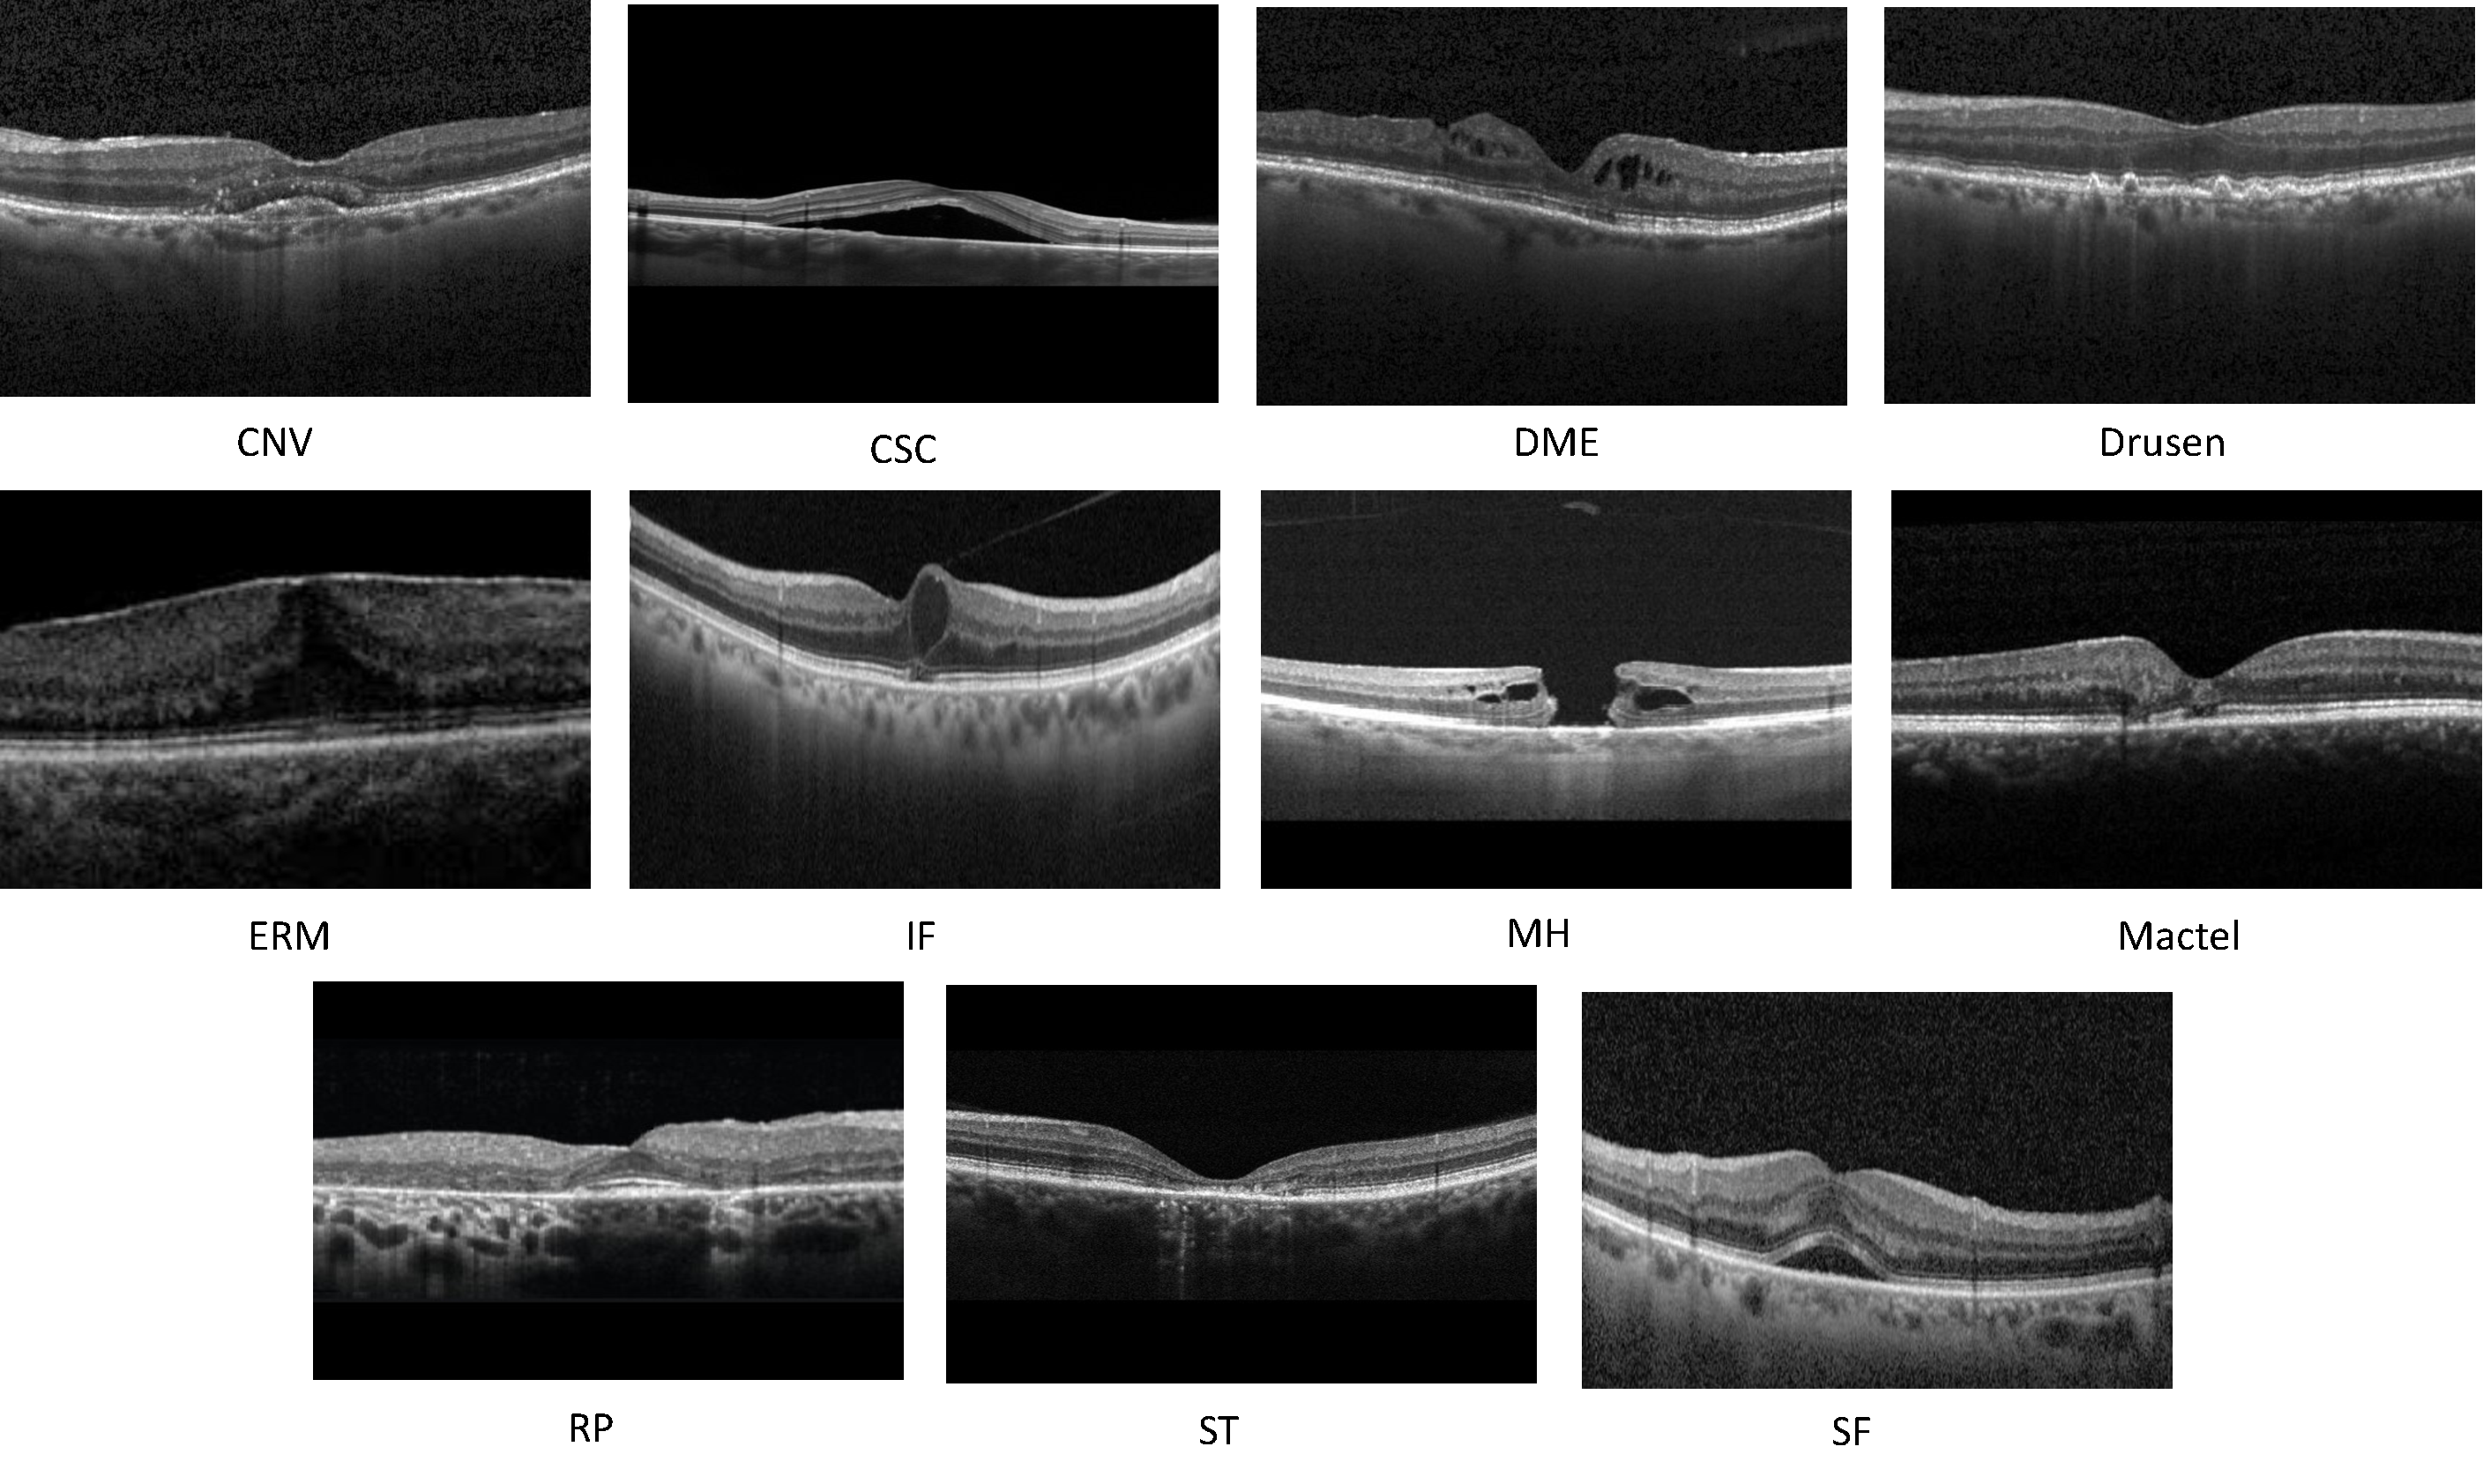
\includegraphics[width=\linewidth]{Figs/OCT_Abnormities.pdf}
		\caption{OCT Abnormities}
		\vspace{0.3cm}
		\label{fig:OCT_abnormities}
	\end{figure}
	
	\begin{figure}[htbp]
		\centering
		\includegraphics[width=\linewidth]{Figs/fundus_Abnormities.pdf}
		\caption{Fundus Abnormities}
		\vspace{0.3cm}
		\label{fig:fundus_abnormities}
	\end{figure}
	
	The Abnormity Models also contain 2 submodels: the OCT Model and the Fundus Model, which classify OCT and fundus abnormities, respectively. Both of the submodels leverage CNNs with modified final fully-connected (FC) layers. We compare the performances of 4 commonly used CNNs, ResNet152, ResNet50, ResNet18 \autocite{He_Zhang_Ren_Sun_2016} and VGG16 \autocite{Simonyan_Zisserman_2015}, and choose the best one for each submodel. The final FC layer in each CNN is modified so that the size of its output vector is equal to the number of OCT or fundus abnormities. In order to normalize the output vector, we perform the softmax operation. Each submodel outputs a probability vector for all the abnormities.
	
	\vspace{0.5cm}
	
	The Diagnosis Model consists of two stages: Stage D1 and Stage D2. 
	
	\vspace{0.2cm}
	
	In Stage D1, we determine the severity level for each disease from the probability vectors from the Abnormity Models. We use Abnormity-to-Disease Deduction Criteria (shown in Fig.~\ref{fig:criteria}) as ground truth. There are multiple submodels in Stage D1 and each one corresponds to one disease. Based on the deduction criteria, we determine the number of abnormities for one disease and use the number to define the severity levels. For example, there are totally 5 abnormities that are present in the disease ``rDR'': OCT abnormity ``DME'' and Fundus abnormities ``HM'', ``VA'', ``MA'', and ``CWP''. Therefore, taking into account the healthy status, we end up with 6 severity levels for disease ``rDR''.

	We use the fused vector as an input for each submodels in Stage D1, and have the vector go through a FC layer with softmax operation to yield severity level probability vectors.
	
	\begin{figure}[htbp]
		\centering
		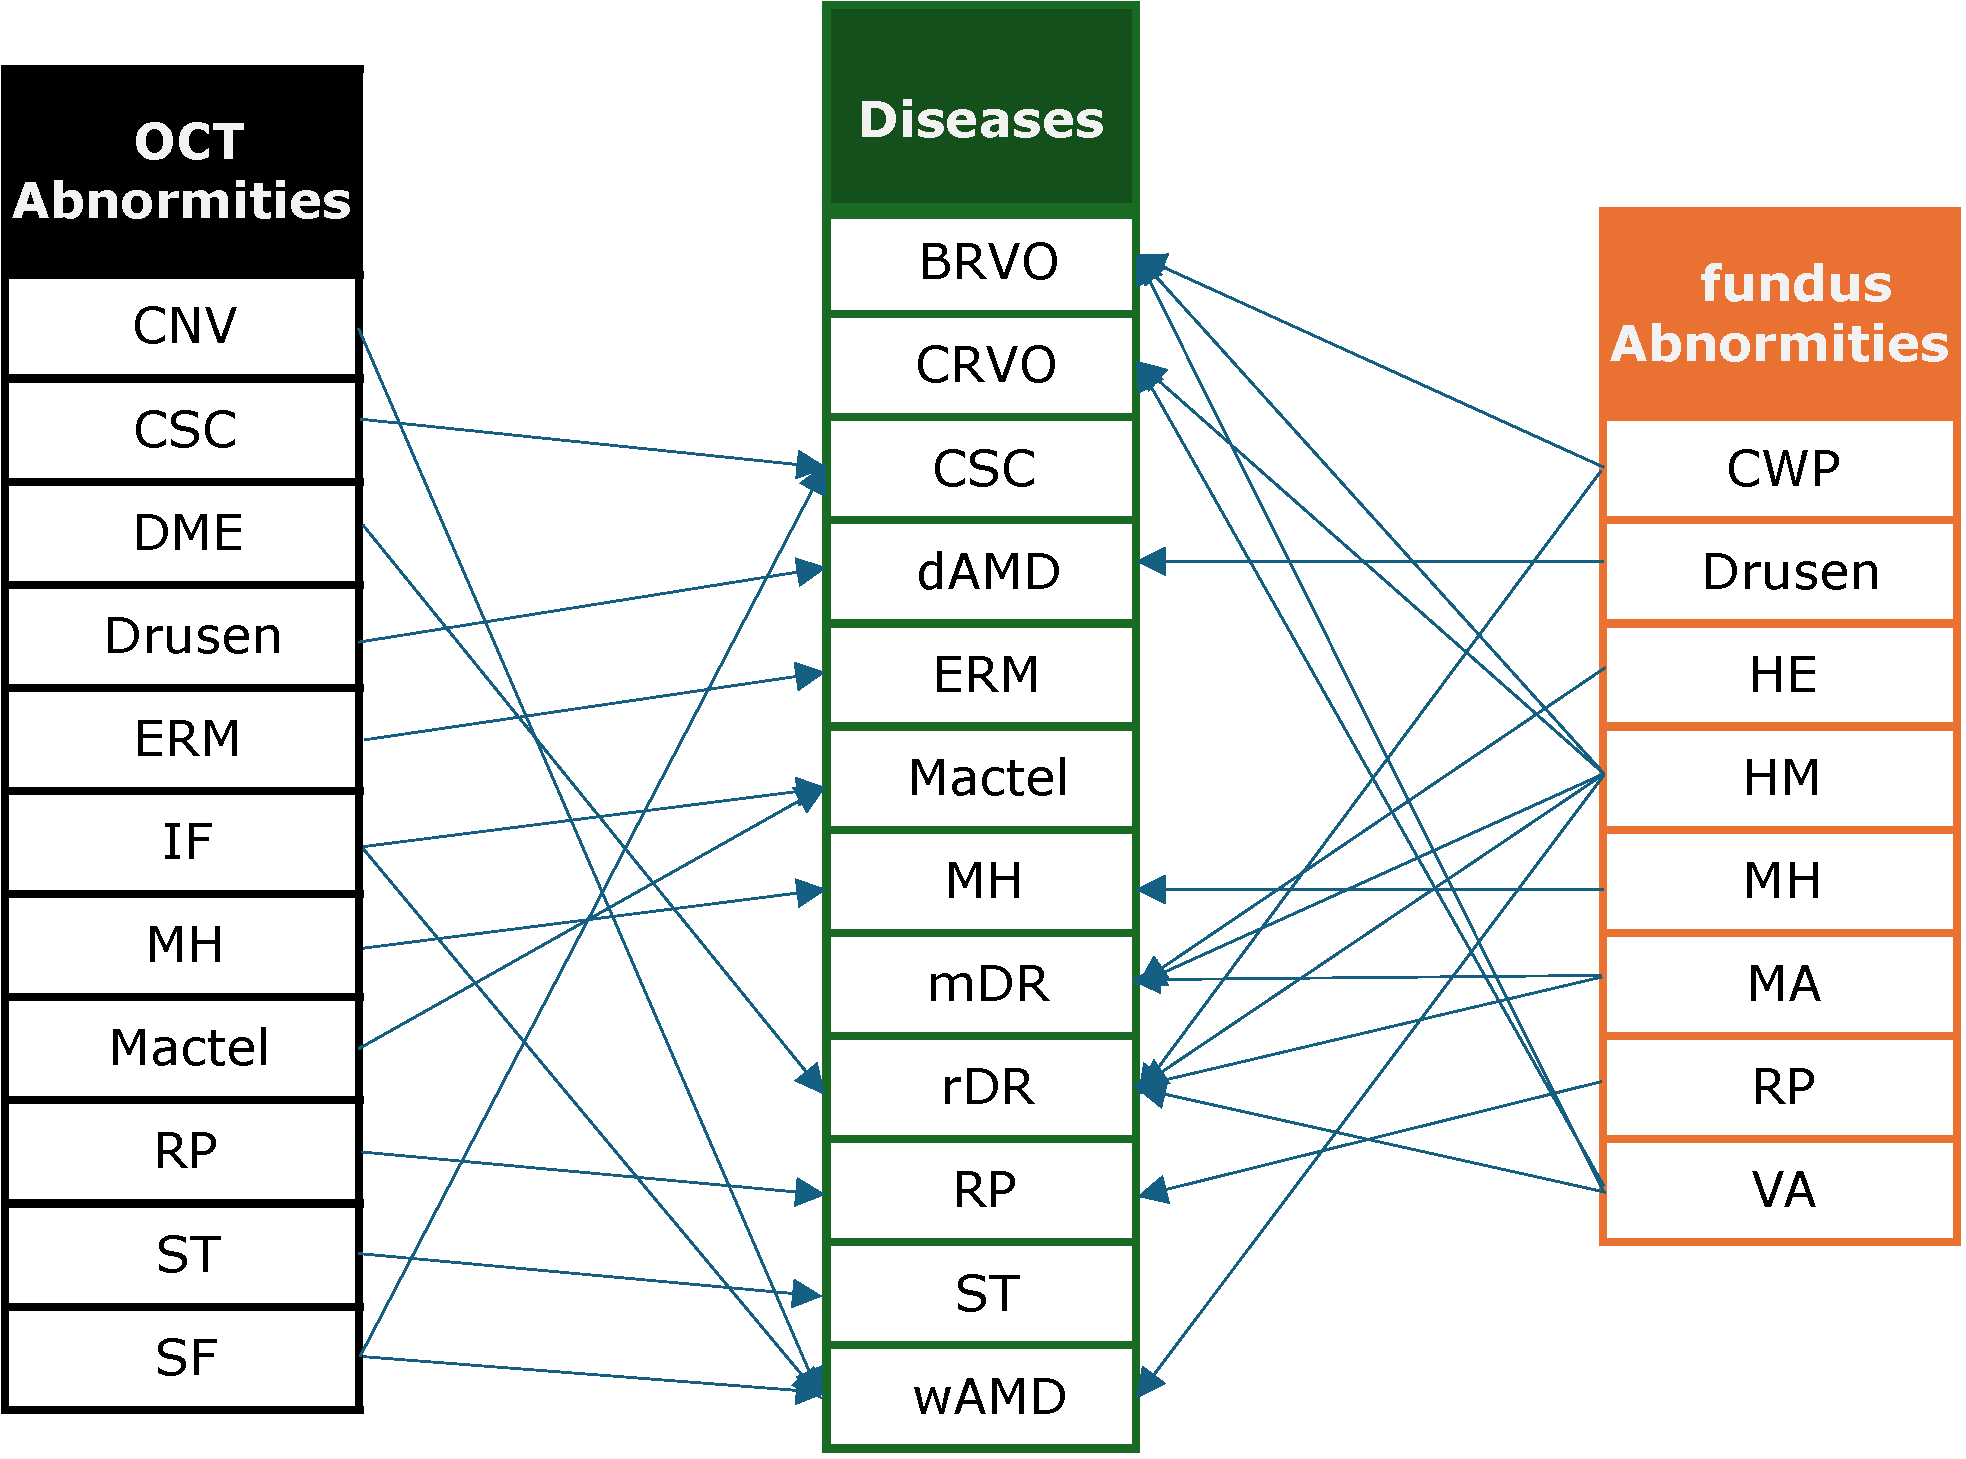
\includegraphics[width=0.8\linewidth]{Figs/criteria.pdf}
		\caption{Abnormity-to-disease Deduction Criteria}
		\vspace{0.3cm}
		\label{fig:criteria}
	\end{figure}

	\vspace{0.2cm}
	
	In Stage D2, we determine the final disease probability vector. Similarly, we use a fused vector from the outputs of submodels in Stage D1, and have the vector go through a FC layer with softmax operation. The result presents potential diseases that can be referenced by ophthalmologists.

	\vspace{0.5cm}
	
	In the MAAM, we leverage the fusion operation to incorporate all the results from different submodels. As shown in Fig.~\ref{fig:fusion}, there are totally 3 fusion operations in MAAM.
	
	\begin{figure}[htbp]
		\centering
		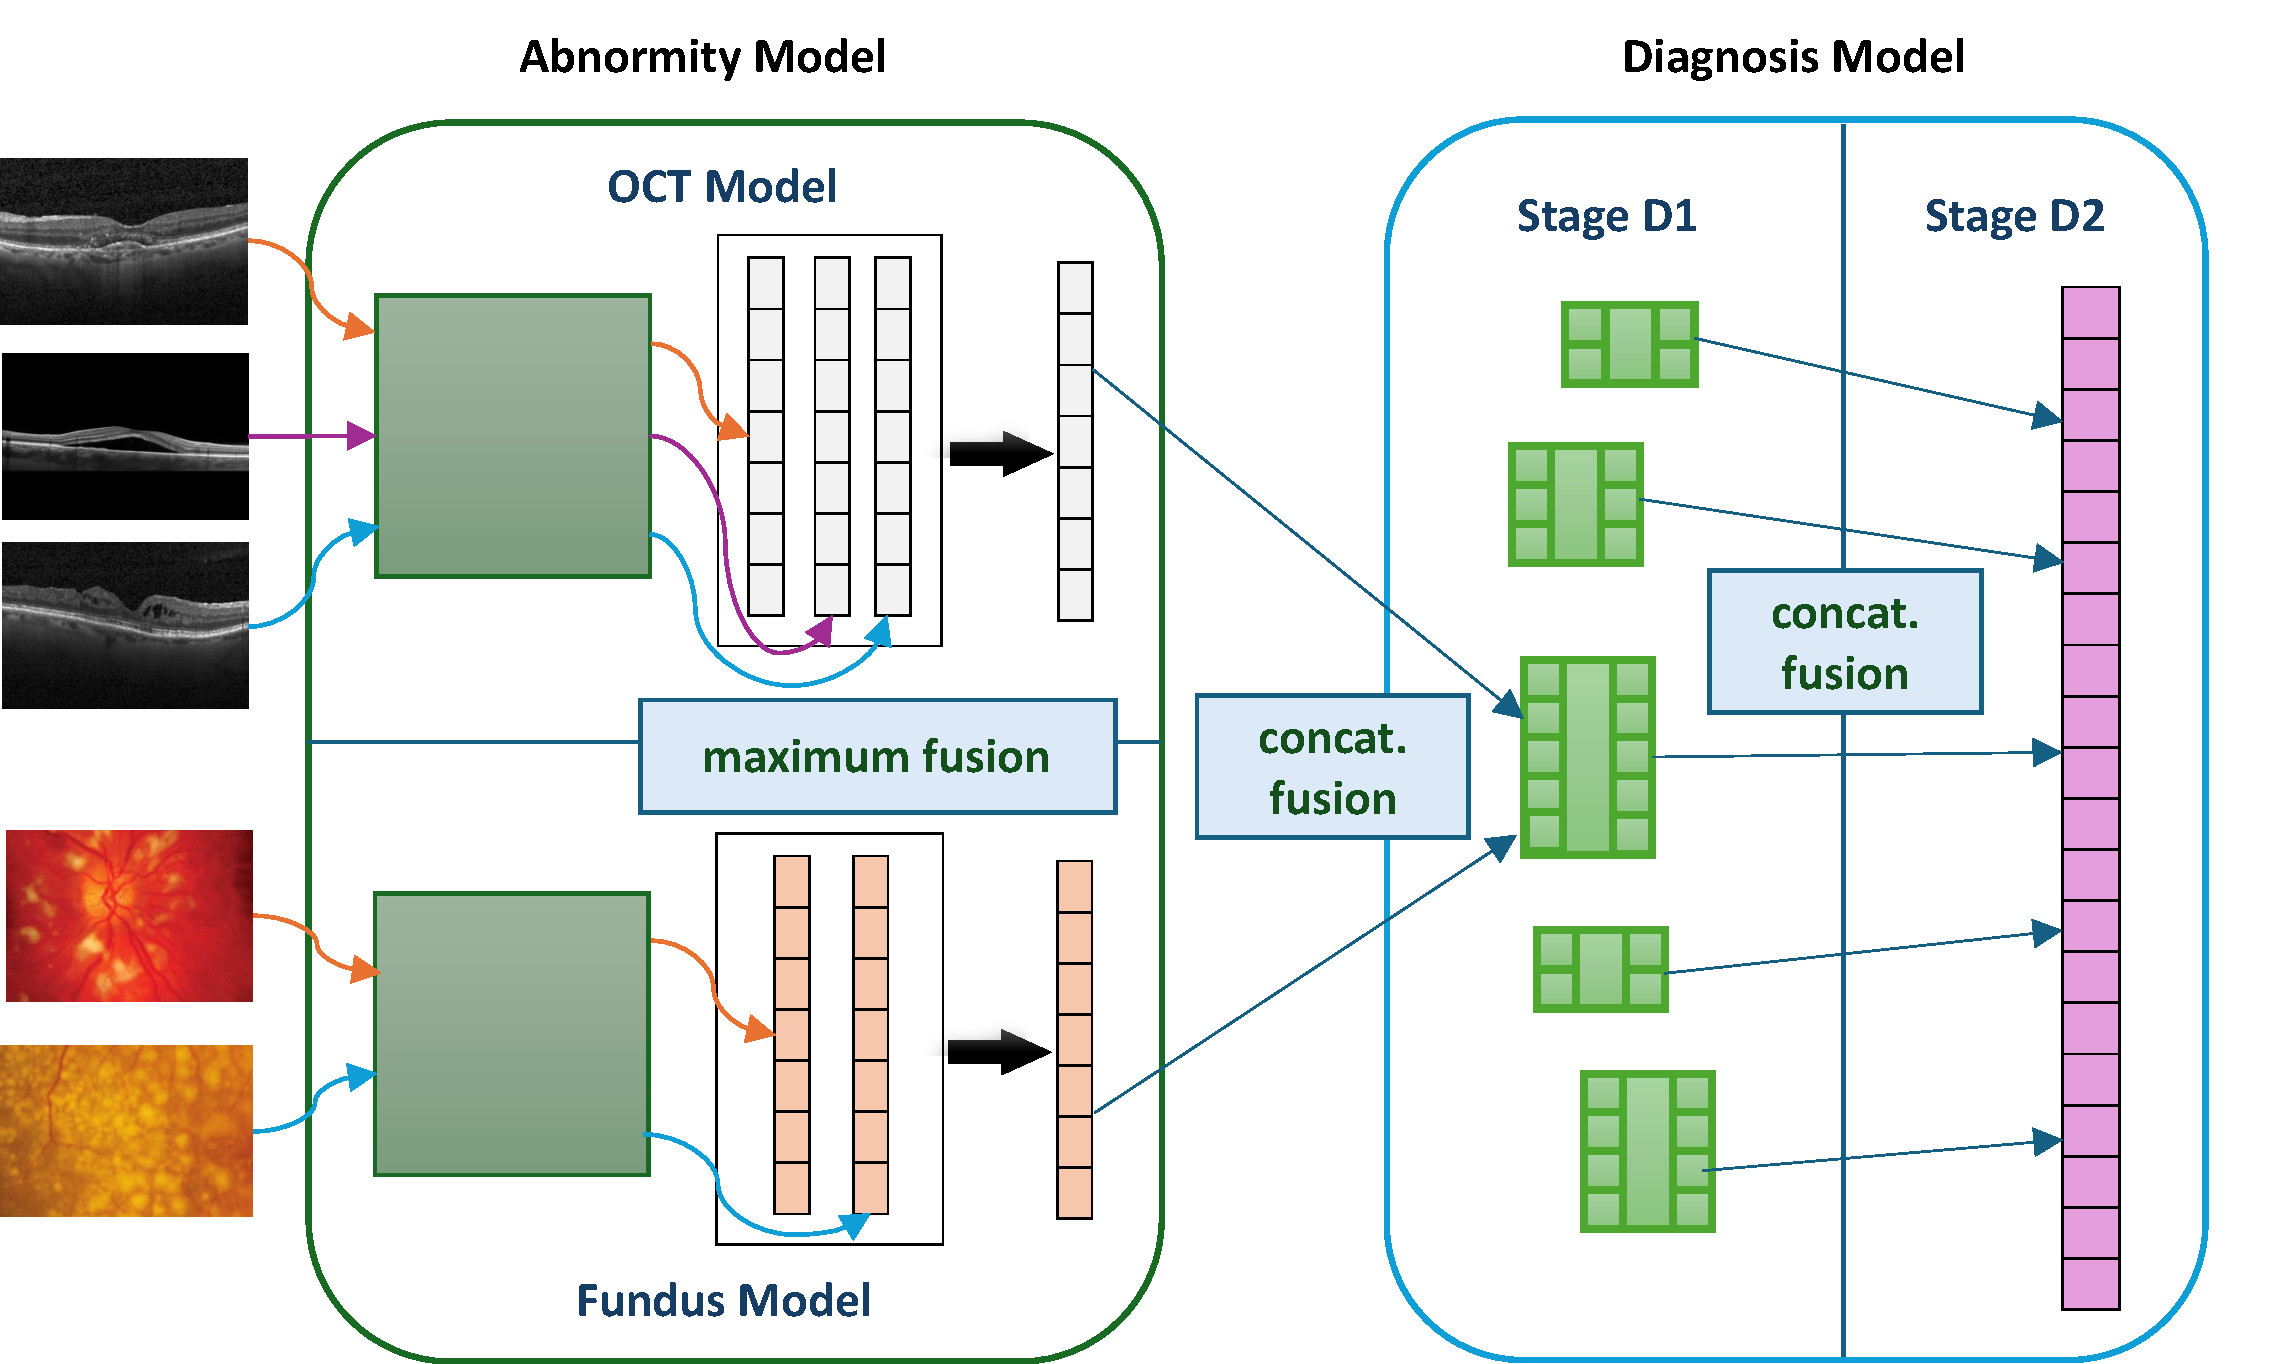
\includegraphics[width=\linewidth]{Figs/fusion.pdf}
		\caption{Fusion}
		\vspace{0.3cm}
		\label{fig:fusion}
	\end{figure}

	The first fusion occurs at the output of OCT Model or Fundus Model. In real scenarios, multiple OCT and Fundus images can be used for ocular disease diagnosis. Each image goes through either the OCT Model or the Fundus Model to yield a probability vector. To use the probability results from all the images, a maximization fusion is implemented for all the vectors so that the fusion yields one OCT abnormity probability vector and one Fundus abnormity probability vector with maximum values.
	
	The second fusion occurs at the interface between Abnormity Model and Stage D1. A concatenation fusion is implemented for OCT abnormity probability vector and Fundus abnormity probability vector. The fused vector works as an input to all the submodels in Stage D1.
	
	The third fusion occurs at the interface between Stage D1 and Stage D2. We concatenation all the severity level vectors to feed the model in Stage D2. The fused vector goes through the FC layer and undergoes a softmax operation to yield the final result.
	
	\section{Abnormity Models}
	
	\subsection{Data Preparation}
	
	The images and labels used for training are mainly downloaded from public databases, but some abnormities are not included in these databases. For those abnormities, we use the search engine as an additional data source to get images. The numbers of images acquired from each data source are shown in Table~\ref{tb:OCT_source} and Table~\ref{tb:Fundus_source}. As to the links of the images from the search engine, refer to ``Appendix''. 
	
	\begin{minipage}[t]{0.4\linewidth}
		{
			\fontsize{9}{12}\selectfont
			{
				\begin{longtable}{cccccc}
					\caption{OCT abnormities}
					\label{tb:OCT_source}\\
					\toprule
					\multirow{2}{*}{Abnormity}&\multicolumn{4}{c}{Source}&\multirow{2}{*}{Total}\\
					&1&2&3&4&\\
					\midrule
					CNV    &2984&/  &/ &/ &2984\\
					CSC    &/   &102&32&/ &134 \\
					DME    &2500&/  &/ &/ &2500\\
					Drusen &2500&/  &/ &/ &2500\\
					ERM    &/   &/  &/ &19&19  \\
					IF     &1097&/  &/ &/ &1097\\
					MH     &/   &99 &31&/ &130 \\
					Mactel &/   &/  &29&/ &29  \\
					Healthy&5000&/  &/ &/ &5000\\
					RP     &/   &102&31&/ &133 \\
					ST     &/   &/  &23&/ &23  \\
					SF     &1083&/  &/ &/ &1083\\
					\bottomrule
				\end{longtable}
				
				\vspace{0.5cm}
				\begin{enumerate}
					\item Normal Disease Database \autocite{Kermany_database}
					\vspace{-0.2cm}
					
					\item OCTID \autocite{Gholami_Roy_Parthasarathy_Lakshminarayanan_2020}
					\vspace{-0.2cm}
					
					\item Few-shot \autocite{Yoo_2020}
					\vspace{-0.2cm}
					
					\item Search engine
					\vspace{-0.2cm}
				\end{enumerate}
				
				\vspace{0.5cm}
			}
		}
	\end{minipage}
	\begin{minipage}[t]{0.6\linewidth}
		{
			\fontsize{9}{12}\selectfont
			{
				\begin{longtable}{cccccccc}
					\caption{Fundus abnormities}
					\label{tb:Fundus_source}\\
					\toprule
					\multirow{2}{*}{Abnormity}&\multicolumn{6}{c}{Source}&\multirow{2}{*}{Total}\\
					&1&2&3&4&5&6&\\
					\midrule
					CWP    &/  &/ &/ &33 &205&/ &238\\
					Drusen &/  &/ &/ &50 &/  &/ &50 \\     
					HE     &20 &/ &/ &75 &284&/ &379\\ 
					HM     &13 &66&/ &105&278&/ &462\\     
					MH     &/  &/ &/ &/  &/  &34&34 \\        
					MA     &55 &/ &/ &1  &219&/ &275\\
					Healthy&100&37&15&/  &/  &/ &152\\      
					RP     &/  &22&/ &/  &/  &44&66 \\         
					VA     &/  &64&/ &14 &/  &/ &78 \\
					
					\bottomrule
				\end{longtable}
				
				\vspace{1cm}
				\begin{enumerate}[left=1.5cm]
					
					\item E-ophtha \autocite{E_ophtha}.
					\vspace{-0.2cm}
					
					\item Kaggle1000 \autocite{1000Fundus_Pytorch_TransferLearning}
					\vspace{-0.2cm}
					
					\item HRF \autocite{HRF_2013}
					\vspace{-0.2cm}
					
					\item STARE \autocite{STARE}
					\vspace{-0.2cm}
					
					\item EyePACS \autocite{DR_dataset}
					\vspace{-0.2cm}
					
					\item Search engine
					\vspace{-0.2cm}
					
				\end{enumerate}
				
				\vspace{0.5cm}
			}
		}
	\end{minipage}
	
	For OCT abnormities with less than 1000 images, we use Cycle-GAN \autocite{Zhu_Park_Isola_Efros_2020} to generate new images. We train a Cycle-GAN network to interconvert healthy and abnormity images, take out the generator that converts healthy to abnormity images, and use it to generate new abnormity images. We go through all generated images and adopt those that clearly display only the abnormity of interest. The adoption rates are shown in Table~\ref{tb:cycleGAN_number}. Fundus images are not generated using Cycle-GAN because generated fundus images are too blurry; in addition, fundus abnormities are usually less salient than OCT ones and cannot be properly learned by Cycle-GAN, given that we only have a small number of fundus images.
	
	{
		\fontsize{9}{12}\selectfont
		{
			\begin{longtable}{ccccc}
				\caption{OCT images CycleGAN adoption rates}
				\label{tb:cycleGAN_number}\\
				\toprule
				Abnormity&Original&Generated&Adopted&Adoption Rate\\
				\midrule
				CSC   &134&3000&1730&58.667\% \\
				ERM   &19 &3000&1931&64.367\% \\
				MH    &130&3000&1811&60.367\% \\
				Mactel&29 &3000&1900&63.333\% \\
				RP    &133&3000&1923&63.100\% \\
				ST    &23 &3000&2572&86.067\% \\
				\bottomrule
			\end{longtable}
		}
	}
	
	We split the images, including generated images, into training and test datasets, and implement a set of transformations on the images, including horizontal flips, random brightness changes from -10\% to +10\%, random horizontal and vertical translations between -5\% and +5\%, random scaling between -20\% and +20\%, and random rotations, which are between -10$^\circ$ and +10$^\circ$ for OCT images and between -30$^\circ$ and +30$^\circ$ for fundus images. The rotation is only applied to images in the train dataset. Eventually, we get 5000 train images and 500 test images for each OCT abnormity, and 3000 train images and 300 test images for each fundus abnormity.
	
	\subsection{Training}
	
	The model training is on a desktop computer with Intel$^®$ Xeon$^®$ Platinum 8352V Processor, 256GB of RAM and 2 NVIDIA GPU (GeForce RTX 4090) with 48GB VRAM. The training uses cross entropy loss, ADAM optimizer with learning rate 0.001, a batch size of 32 and five-fold cross-validation. The code is written with PyTorch in an Anaconda environment. Refer to ``Appendix'' for the link to the code repository on GitHub. 
	
	\vspace{0.3cm}
	
	For the Abnormity Models, we employ a strategy of transfer learning to finetuning. 
	
	In the transfer learning phase, pretrained weights from ImageNet \autocite{Krizhevsky_Sutskever_Hinton_2017} are used. We freeze the weights in all the convolutional layers and only vary the weights in the final FC layer. The training lasts for 100 epochs. Every 10 epochs, weights of the model with the best validation accuracy are saved. In order to prevent overfitting on the train dataset, we introduce a measure called overall accuracy, which is the weighted average of validation and test accuracy. For all the saved models, we calculate the overall accuracy to select the model with the best overall performance on the validation and test datasets, and start finetuning based on this model. 
	
	In the finetuning phase, we start from the best model in the transfer learning phase, unfreezing all weights in the model. We train the model for 30 epochs. Similarly, we save the weights of the model with the best validation accuracy every 10 epochs, and find the model with the highest overall accuracy. Finally, we compare the overall accuracies of the best model in the transfer learning phase and the finetuning phase to determine the best model of all. 
	
	For both OCT and Fundus Models, we trained 4 commonly used CNNs: ResNet152, ResNet50, ResNet18, and VGG16. The accuracies and losses during training and validation phases are shown in Fig.~\ref{fig:AO_train} and Fig.~\ref{fig:AF_train}. 
	
	\begin{figure}[htbp]
		\centering
		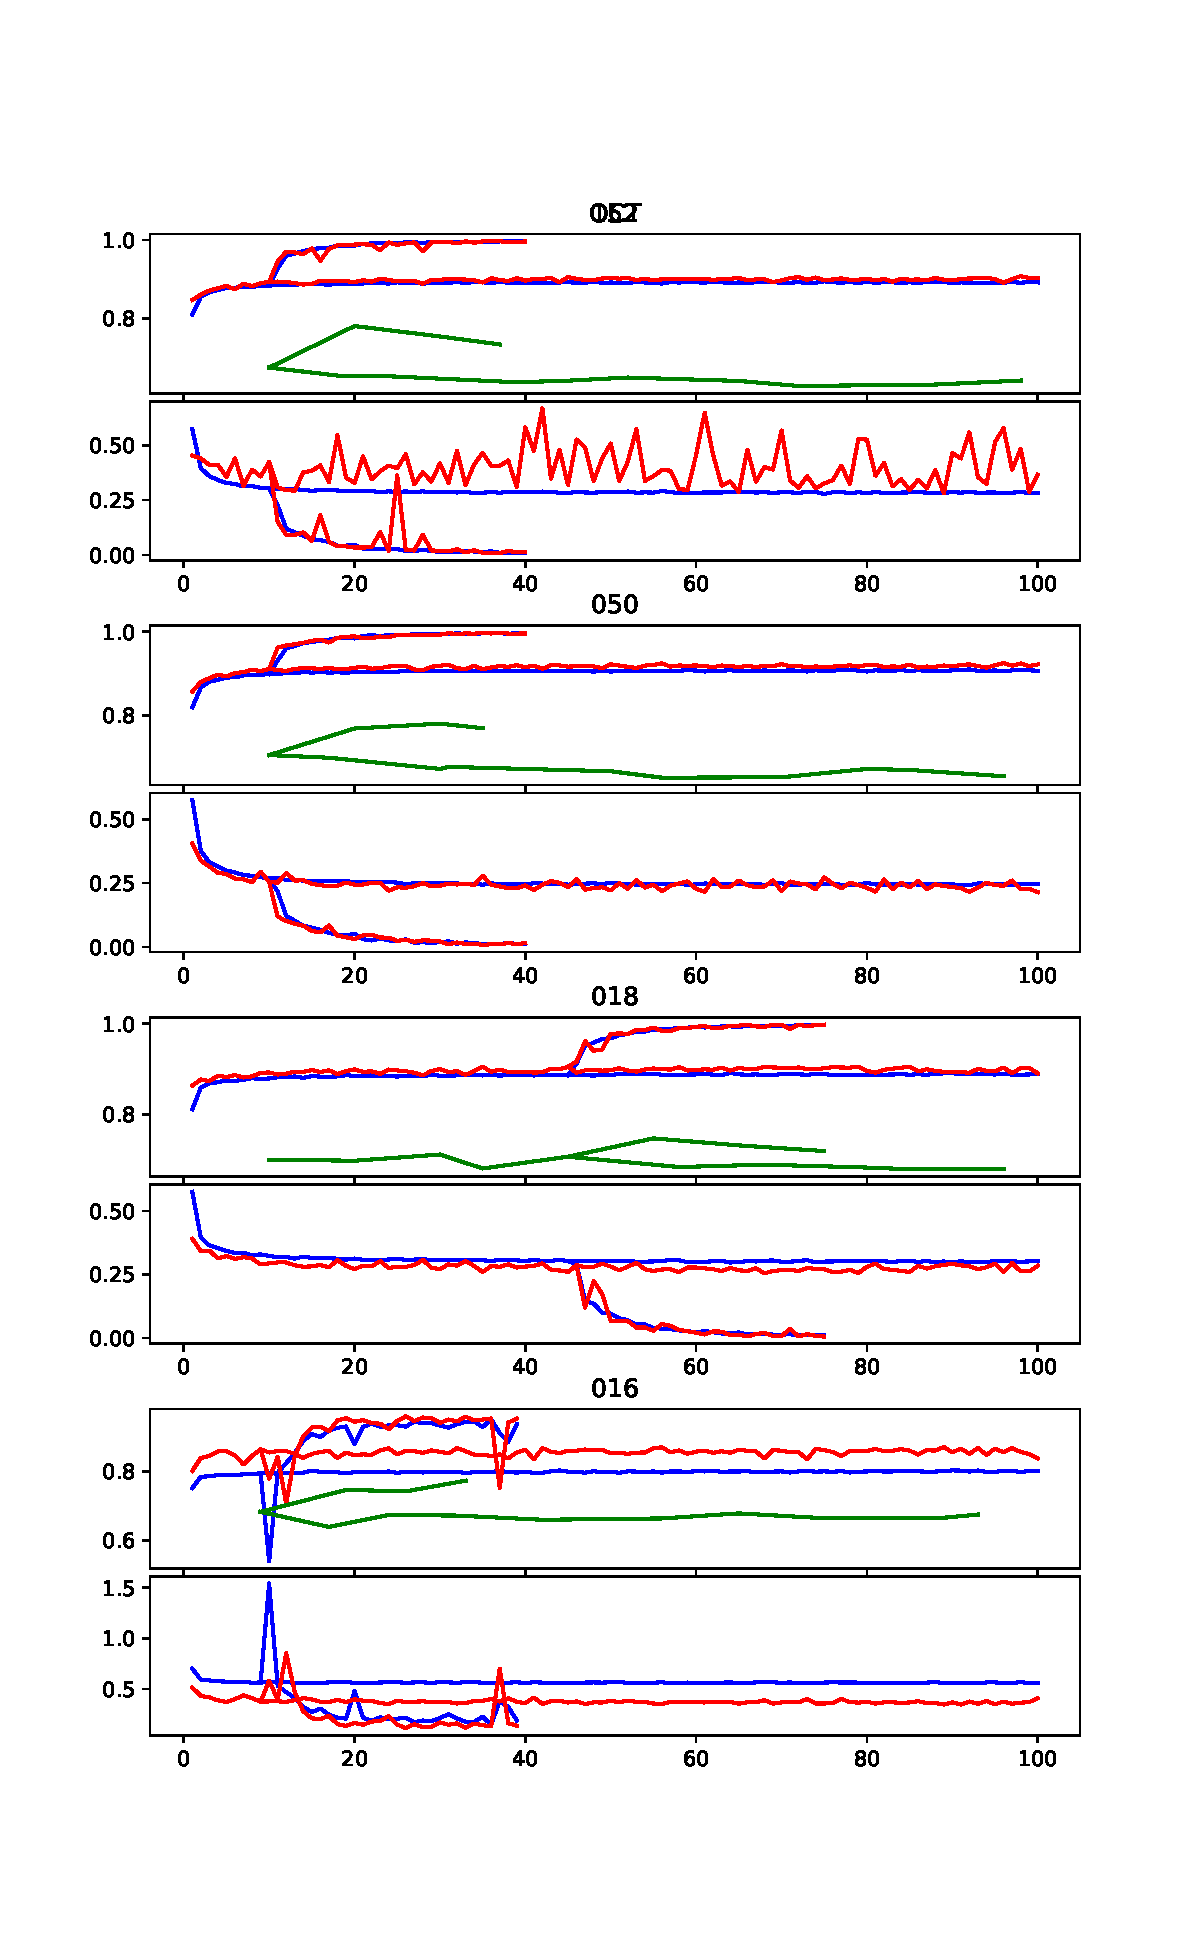
\includegraphics[width=\linewidth]{Figs/abnormity_OCT_loss_and_acc.pdf}
		\caption{AO train}
		\vspace{0.3cm}
		\label{fig:AO_train}
	\end{figure}
	
	\begin{figure}[htbp]
		\centering
		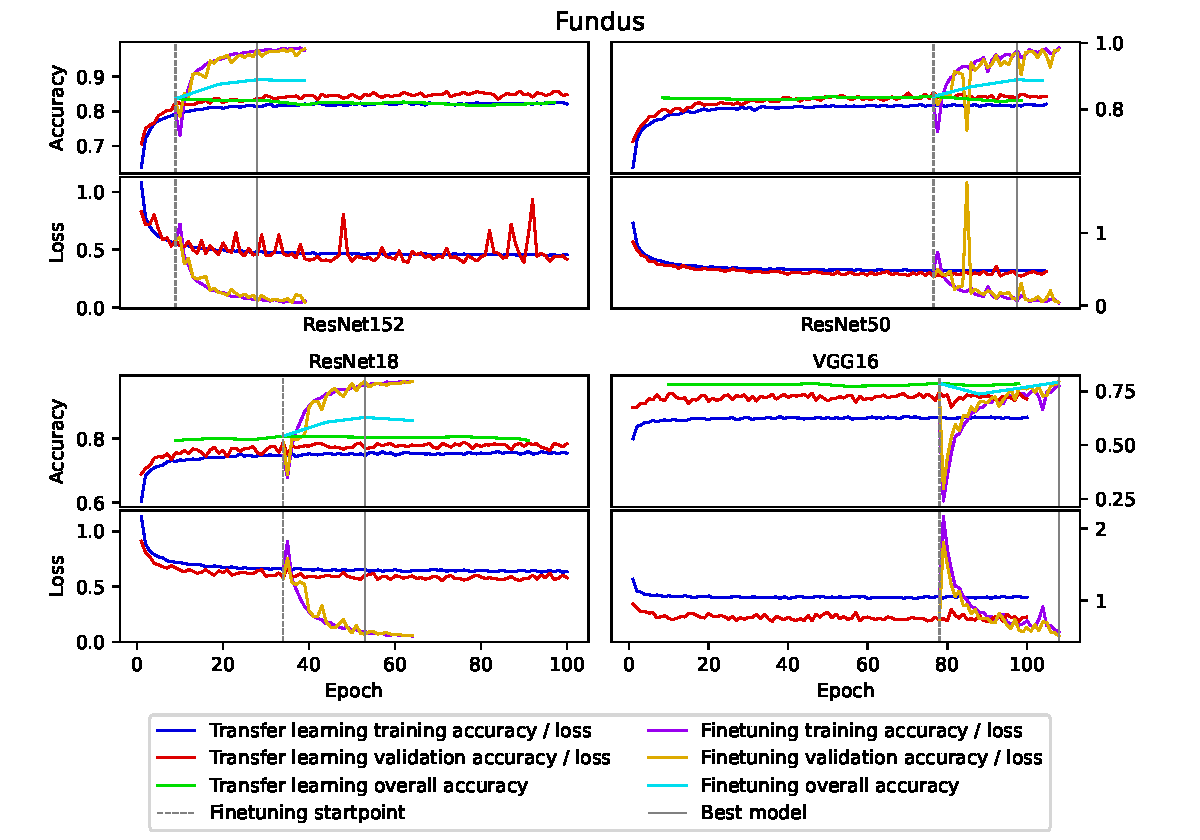
\includegraphics[width=\linewidth]{Figs/abnormity_Fundus_loss_and_acc.pdf}
		\caption{AF train}
		\vspace{0.3cm}
		\label{fig:AF_train}
	\end{figure}
	
	\vspace{0.3cm}
	
	We can observe that finetuning significantly increases the model accuracy and, therefore, all the final models are finetuned models. As shown in Table~\ref{tb:A_accuracies}, the best CNN for OCT Model is ResNet50 and the best for Fundus Model is ResNet152. ResNet50 performed better than ResNet152 on OCT, possibly because it has fewer parameters and is less likely to overfit on OCT images, which has fewer and clearer traits; on the other hand, ResNet152 is better on fundus possibly because it has more parameters and can better discern the complex traits in fundus images. ResNet18 may have too few parameters, so it performs less well over all; and VGG16 sometimes experiences large dips in accuracy, possibly due to gradient vanishing, and this impairs its performance. 
	
	\vspace{0.2cm}
	
	After all the training and comparisons, we determine to use a finetuned model with ResNet50 for OCT Model and a finetuned model with ResNet152 for Fundus Model. 
	
	{
		\fontsize{9}{12}\selectfont
		{
			\begin{table}
				\centering
				\caption{Validation accuracies}
				\label{tb:A_accuracies}
				\begin{tabular}{ccccc}
					\toprule
					Model&ResNet152&ResNet50&ResNet18&VGG16\\
					\midrule
					OCT Model   &91.906\%&\textbf{92.183\%}&91.011\%&89.744\% \\
					Fundus Model&\textbf{89.111\%}&88.926\%&86.605\%&79.185\% \\
					\bottomrule
				\end{tabular}
			\end{table}
		}
	}
	
	\subsection{Results}
	
	Table~\ref{tb:OCT_test} and Table~\ref{tb:Fundus_test} show the predictive values on the test dataset. Fig.~\ref{fig:A_ROC} shows the ROCs of each abnormity. The results show that the performance of the OCT Model is significantly better than that of the Fundus Model. Fundus abnormities tend to be less prominent, since the abnormity on fundus image are usually quite small and scattered. Moreover, one fundus image usually contains more than one abnormities, while most OCT images contain only one abnormity on each image. Also given that we have less fundus images than OCT ones, the difficulties for fundus classification increases.
	
	\begin{table}[htbp]
		\centering
		\caption{OCT Test}
		\label{tb:OCT_test}
		\pgfplotstabletypeset[
		multicolumn names,
		col sep=comma,
		columns = {Abnormity, Precision, Sensitivity, Specificity, FOne, AUC},
		columns/Abnormity/.style={string type, column name=Abnormities},
		columns/Precision/.style={string type, column name=Precision},
		columns/Sensitivity/.style={string type, column name=Sensitivity},
		columns/Specificity/.style={string type, column name=Specificity},
		columns/FOne/.style={string type, column name={F1 Score}},
		columns/AUC/.style={string type, column name=AUC},
		every head row/.style={before row=\toprule, after row=\midrule},
		every last row/.style={ after row=\bottomrule}
		]{Tables/abnormity_o_test.csv}
	\end{table}
	
	\begin{table}[htbp]
		\centering
		\caption{Fundus Test}
		\label{tb:Fundus_test}
		\pgfplotstabletypeset[
		multicolumn names,
		col sep=comma,
		columns = {Abnormity, Precision, Sensitivity, Specificity, FOne, AUC},
		columns/Abnormity/.style={string type, column name=Abnormities},
		columns/Precision/.style={string type, column name=Precision},
		columns/Sensitivity/.style={string type, column name=Sensitivity},
		columns/Specificity/.style={string type, column name=Specificity},
		columns/FOne/.style={string type, column name={F1 Score}},
		columns/AUC/.style={string type, column name=AUC},
		every head row/.style={before row=\toprule, after row=\midrule},
		every last row/.style={after row=\bottomrule}
		]{Tables/abnormity_f_test.csv}
	\end{table}
	
	\begin{figure}[htbp]
		\centering
		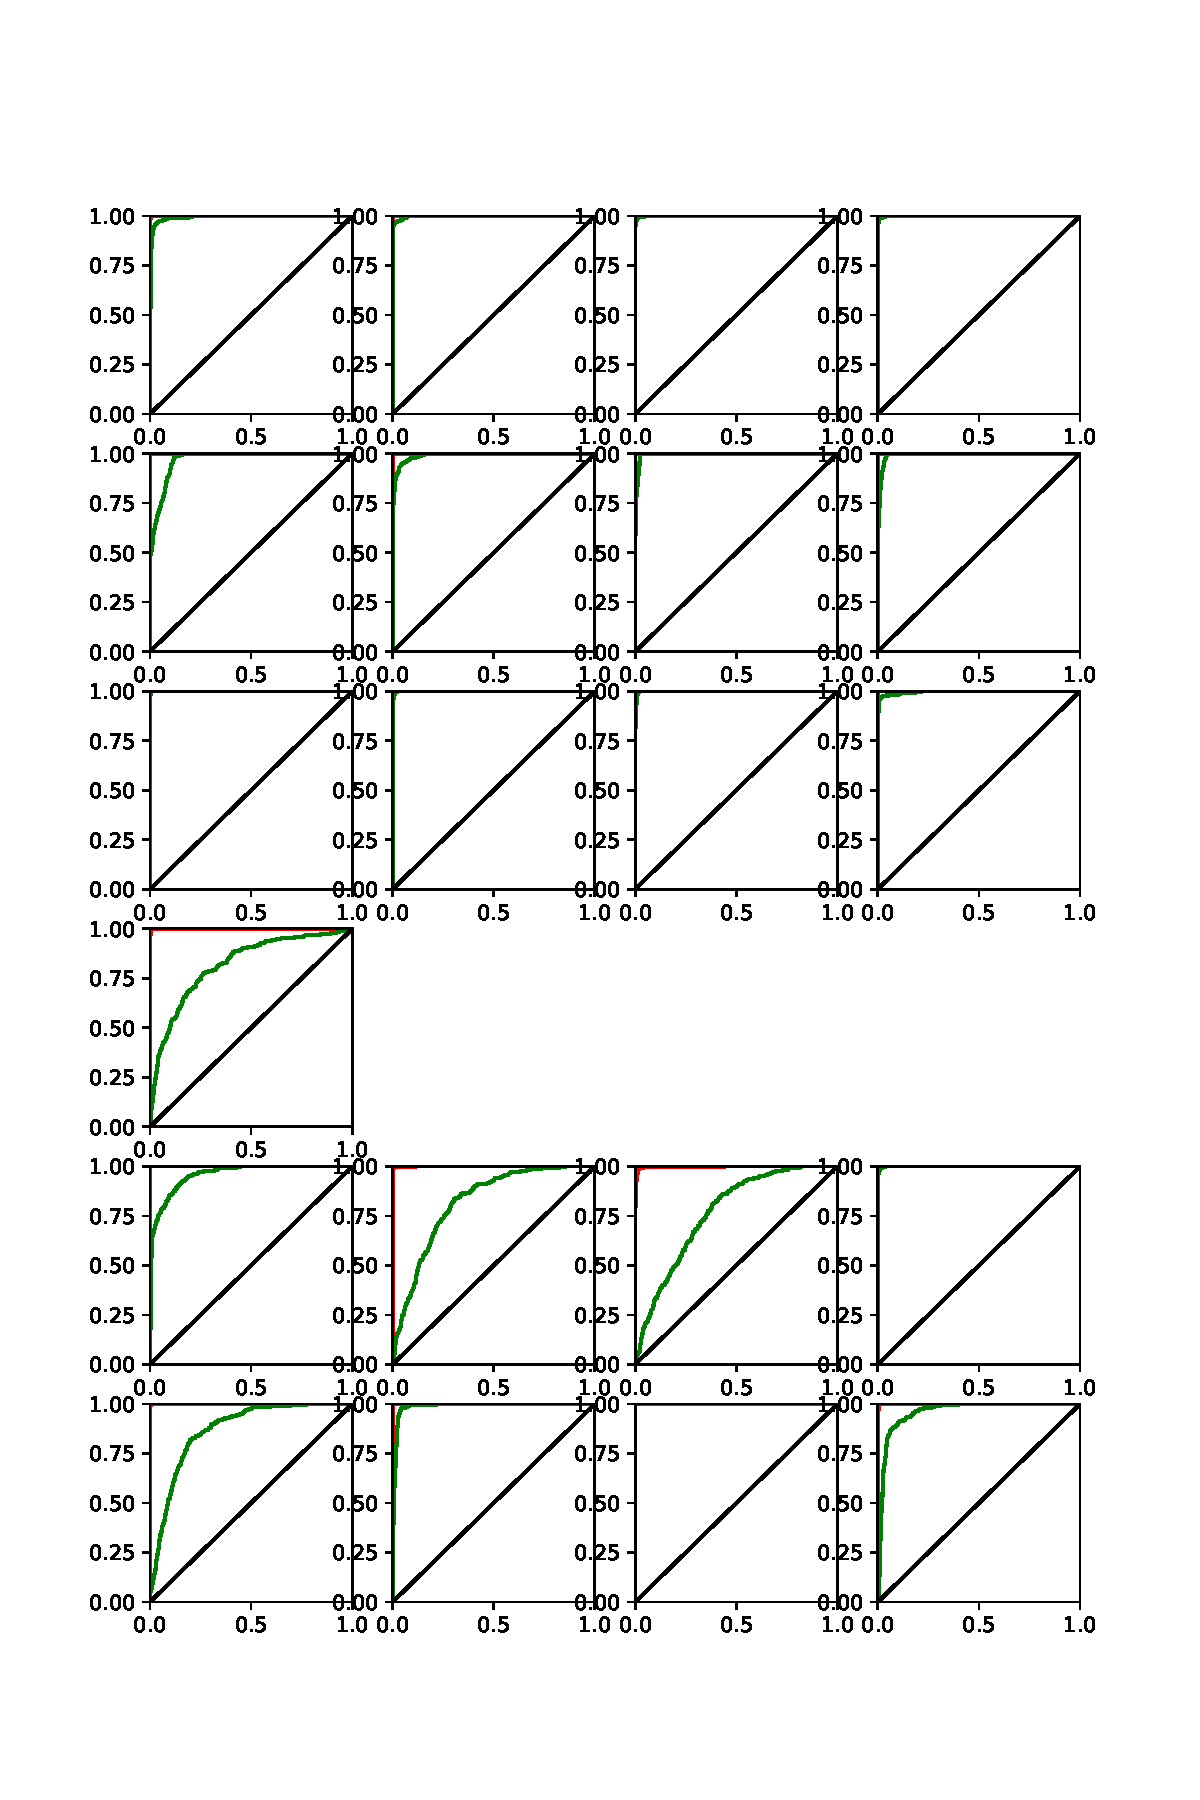
\includegraphics[width=\linewidth]{Figs/abnormity_ROC.pdf}
		\caption{A ROC}
		\vspace{0.3cm}
		\label{fig:A_ROC}
	\end{figure}
	
	The confusion matrices are shown in Fig.~\ref{fig:A_conf_mat}) and the t-SNE graphs are shown in Fig.~\ref{fig:A_tSNE}. During training, most of the abnormities are well-separated. However, this is not the case during testing. On the t-SNE graph, the OCT Model still shows clear separation of clusters, many of which, however, are mingled with data points that do not belong to the cluster. This is because some OCT abnormities resemble each other. For example, ``IF'', ``DME'' and ``Mactel'' may look very similar. As to the Fundus Model, there are fewer small distinct clusters and there is a large cluster instead. This is likely due to the fact that many fundus images contain multiple abnormities. For example, a patient with the disease ``rDR'' shows the abnormities ``CWP'', ``HE'', ``HM'' and ``VA''. Therefore, many abnormities tend to appear together, impeding classification of abnormities. 
	
	\begin{figure}[htbp]
		\centering
		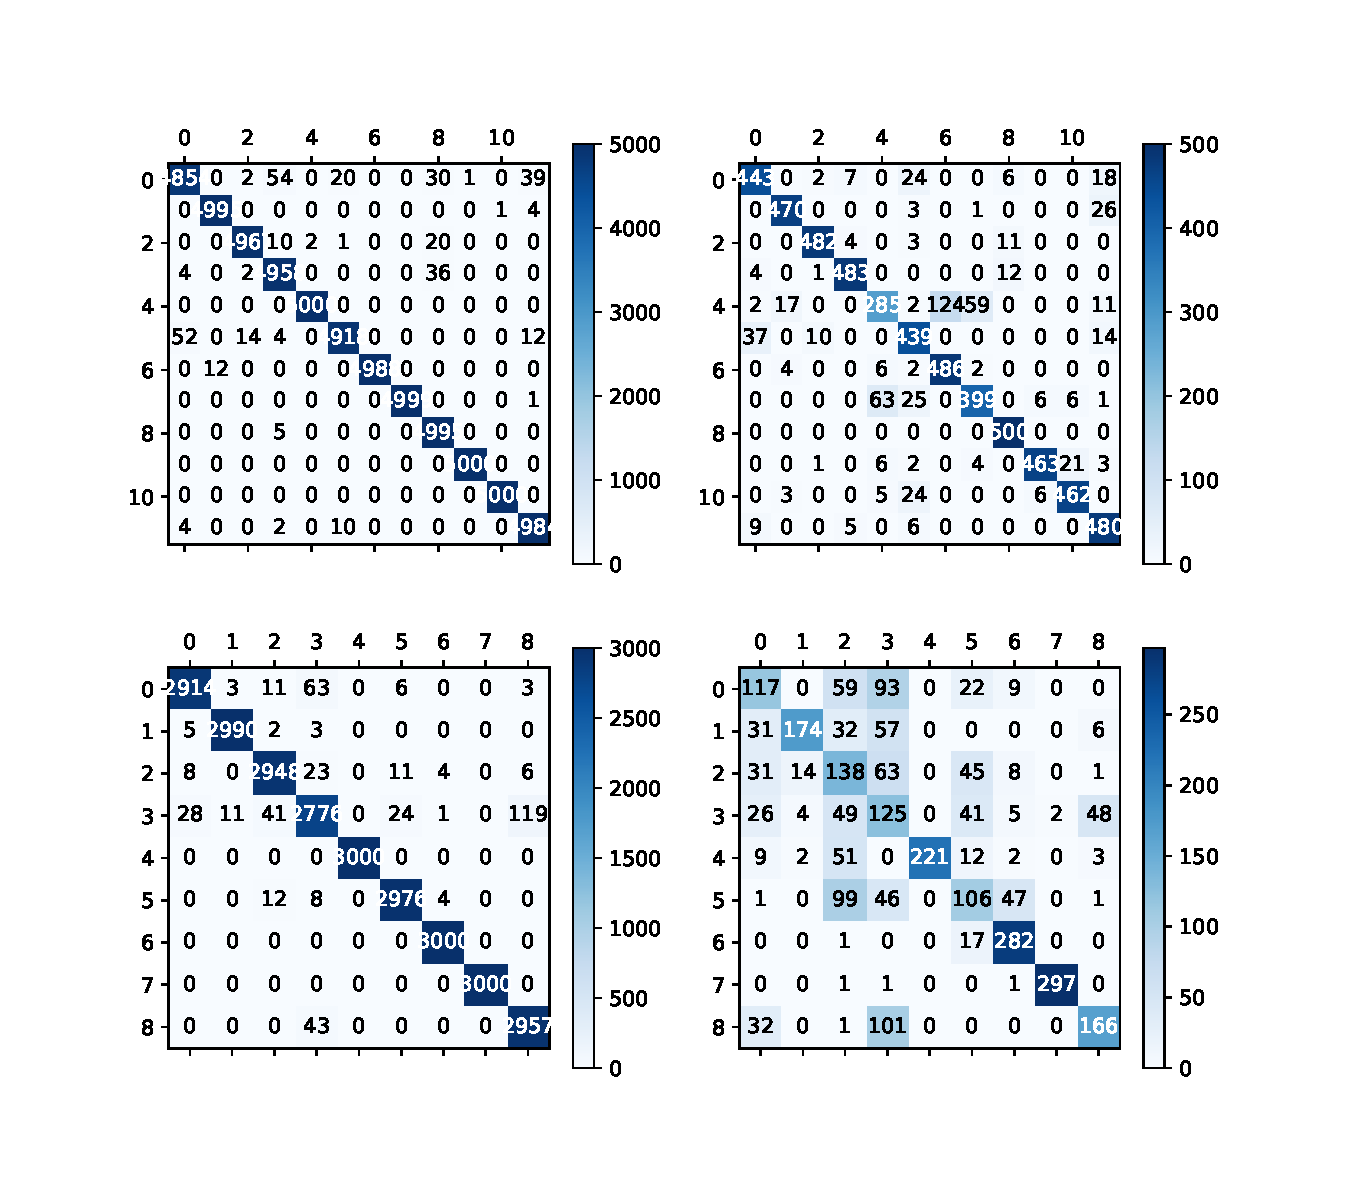
\includegraphics[width=0.8\linewidth]{Figs/abnormity_confusion_matrix.pdf}
		\caption{A Conf Mat}
		\vspace{0.3cm}
		\label{fig:A_conf_mat}
	\end{figure}
	
	\begin{figure}[htbp]
		\centering
		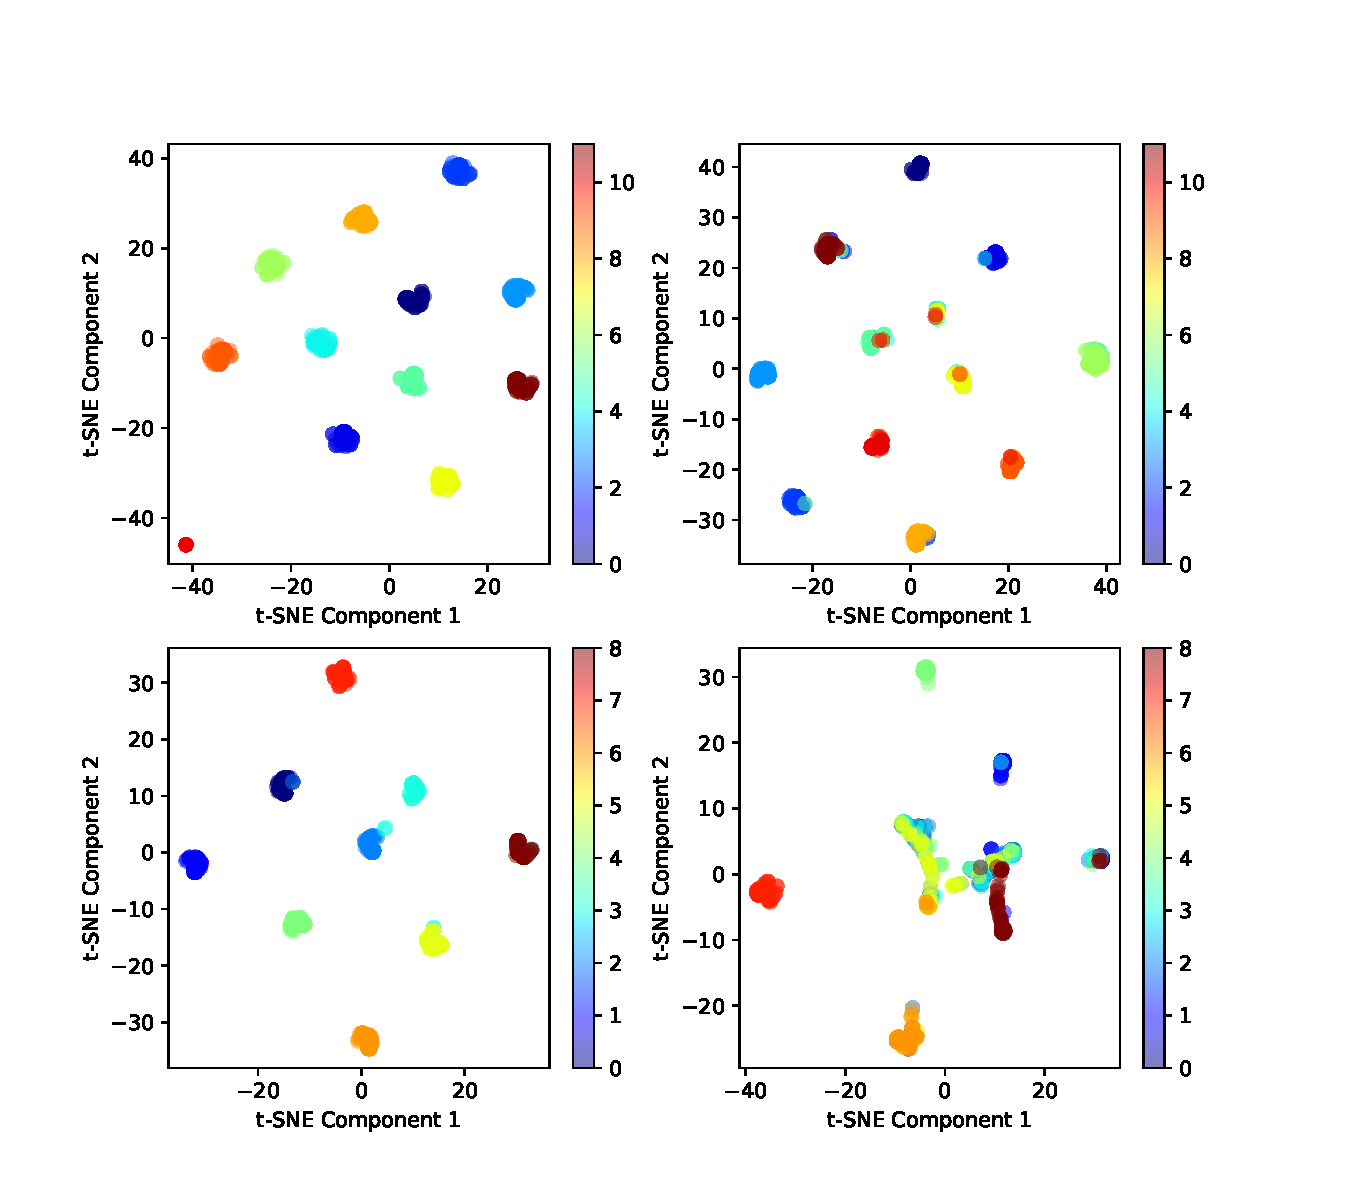
\includegraphics[width=\linewidth]{Figs/abnormity_tSNE.pdf}
		\caption{A ROC}
		\vspace{0.3cm}
		\label{fig:A_tSNE}
	\end{figure}
	
	We can use Grad-CAM \autocite{Selvaraju_Cogswell_Das_Vedantam_Parikh_Batra} to highlight areas on the image that make a large contribution to the final classification. If the model had been trained correctly, this would be equivalent to highlighting the abnormity. Fig.~\ref{fig:gradCAM} shows some examples. Furthermore, Grad-CAM can highlight a designated abnormity, so it may be able to highlight multiple abnormities on one image, as shown in Fig.~\ref{fig:gradCAM_multi_abnormity}. 
	
	\begin{figure}[htbp]
		\centering
		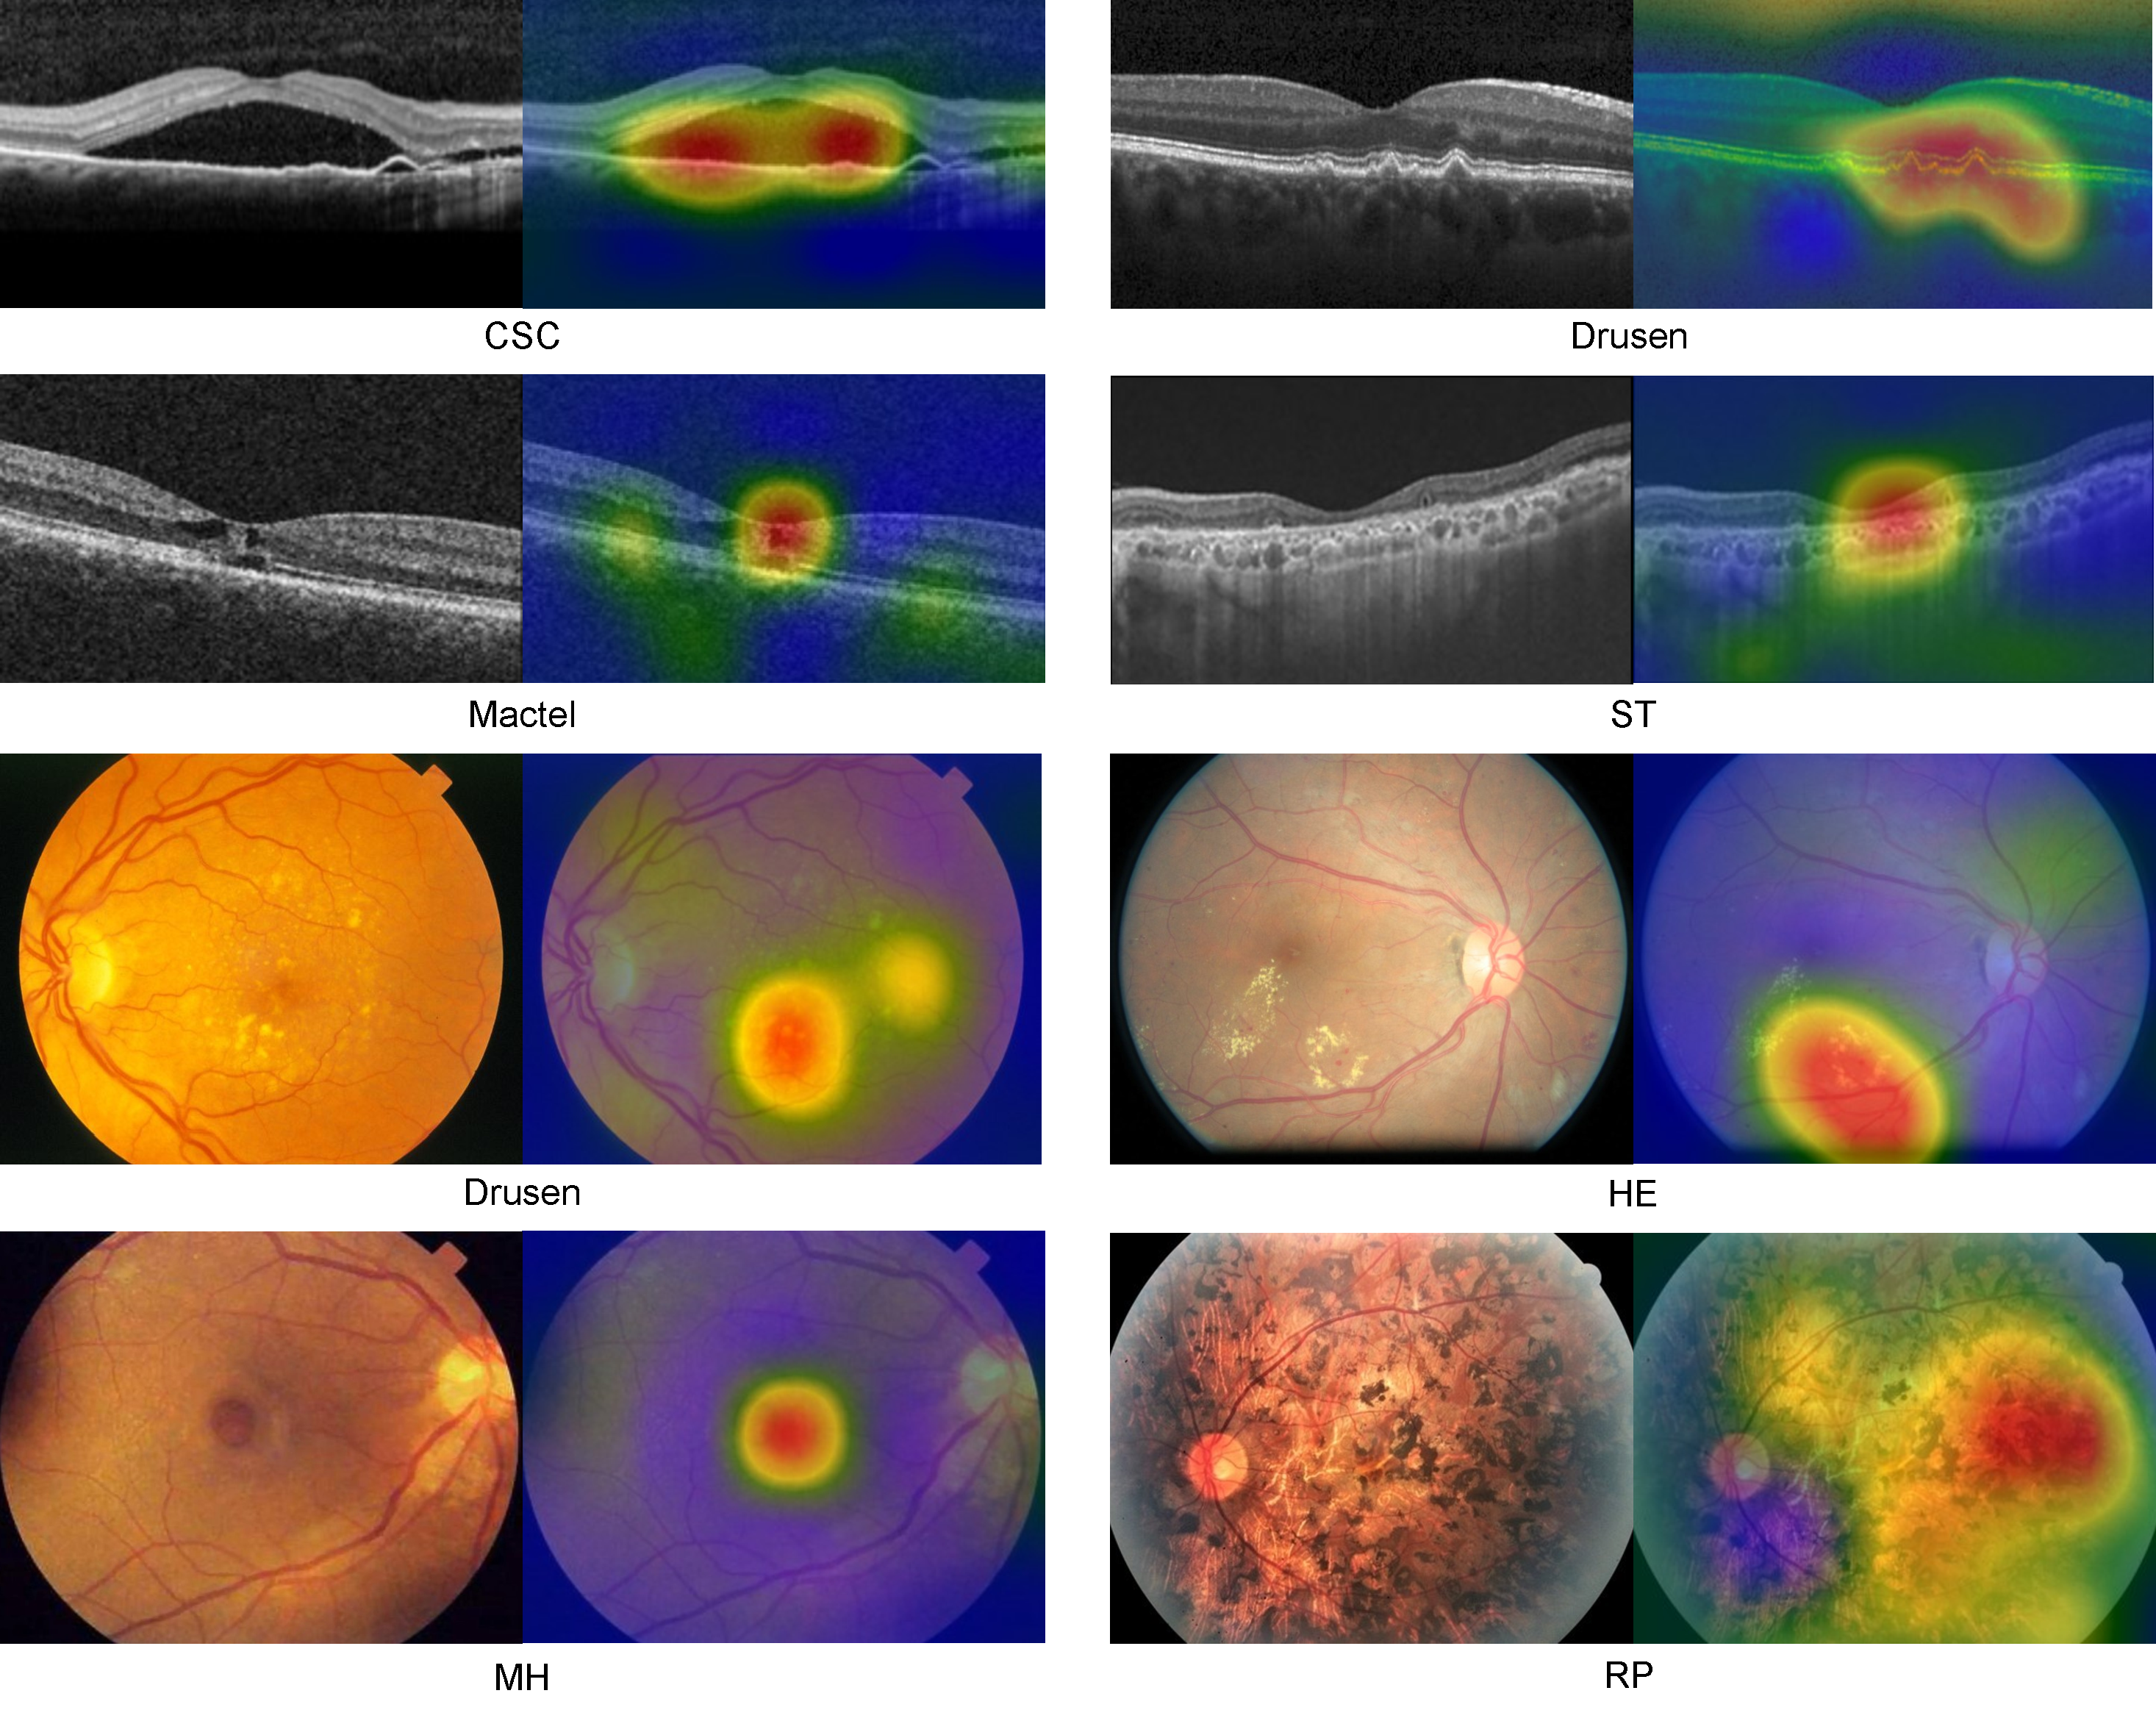
\includegraphics[width=\linewidth]{Figs/abnormity_gradCAM.pdf}
		\caption{GradCAM}
		\vspace{0.3cm}
		\label{fig:gradCAM}
	\end{figure}
	
	\begin{figure}[htbp]
		\centering
		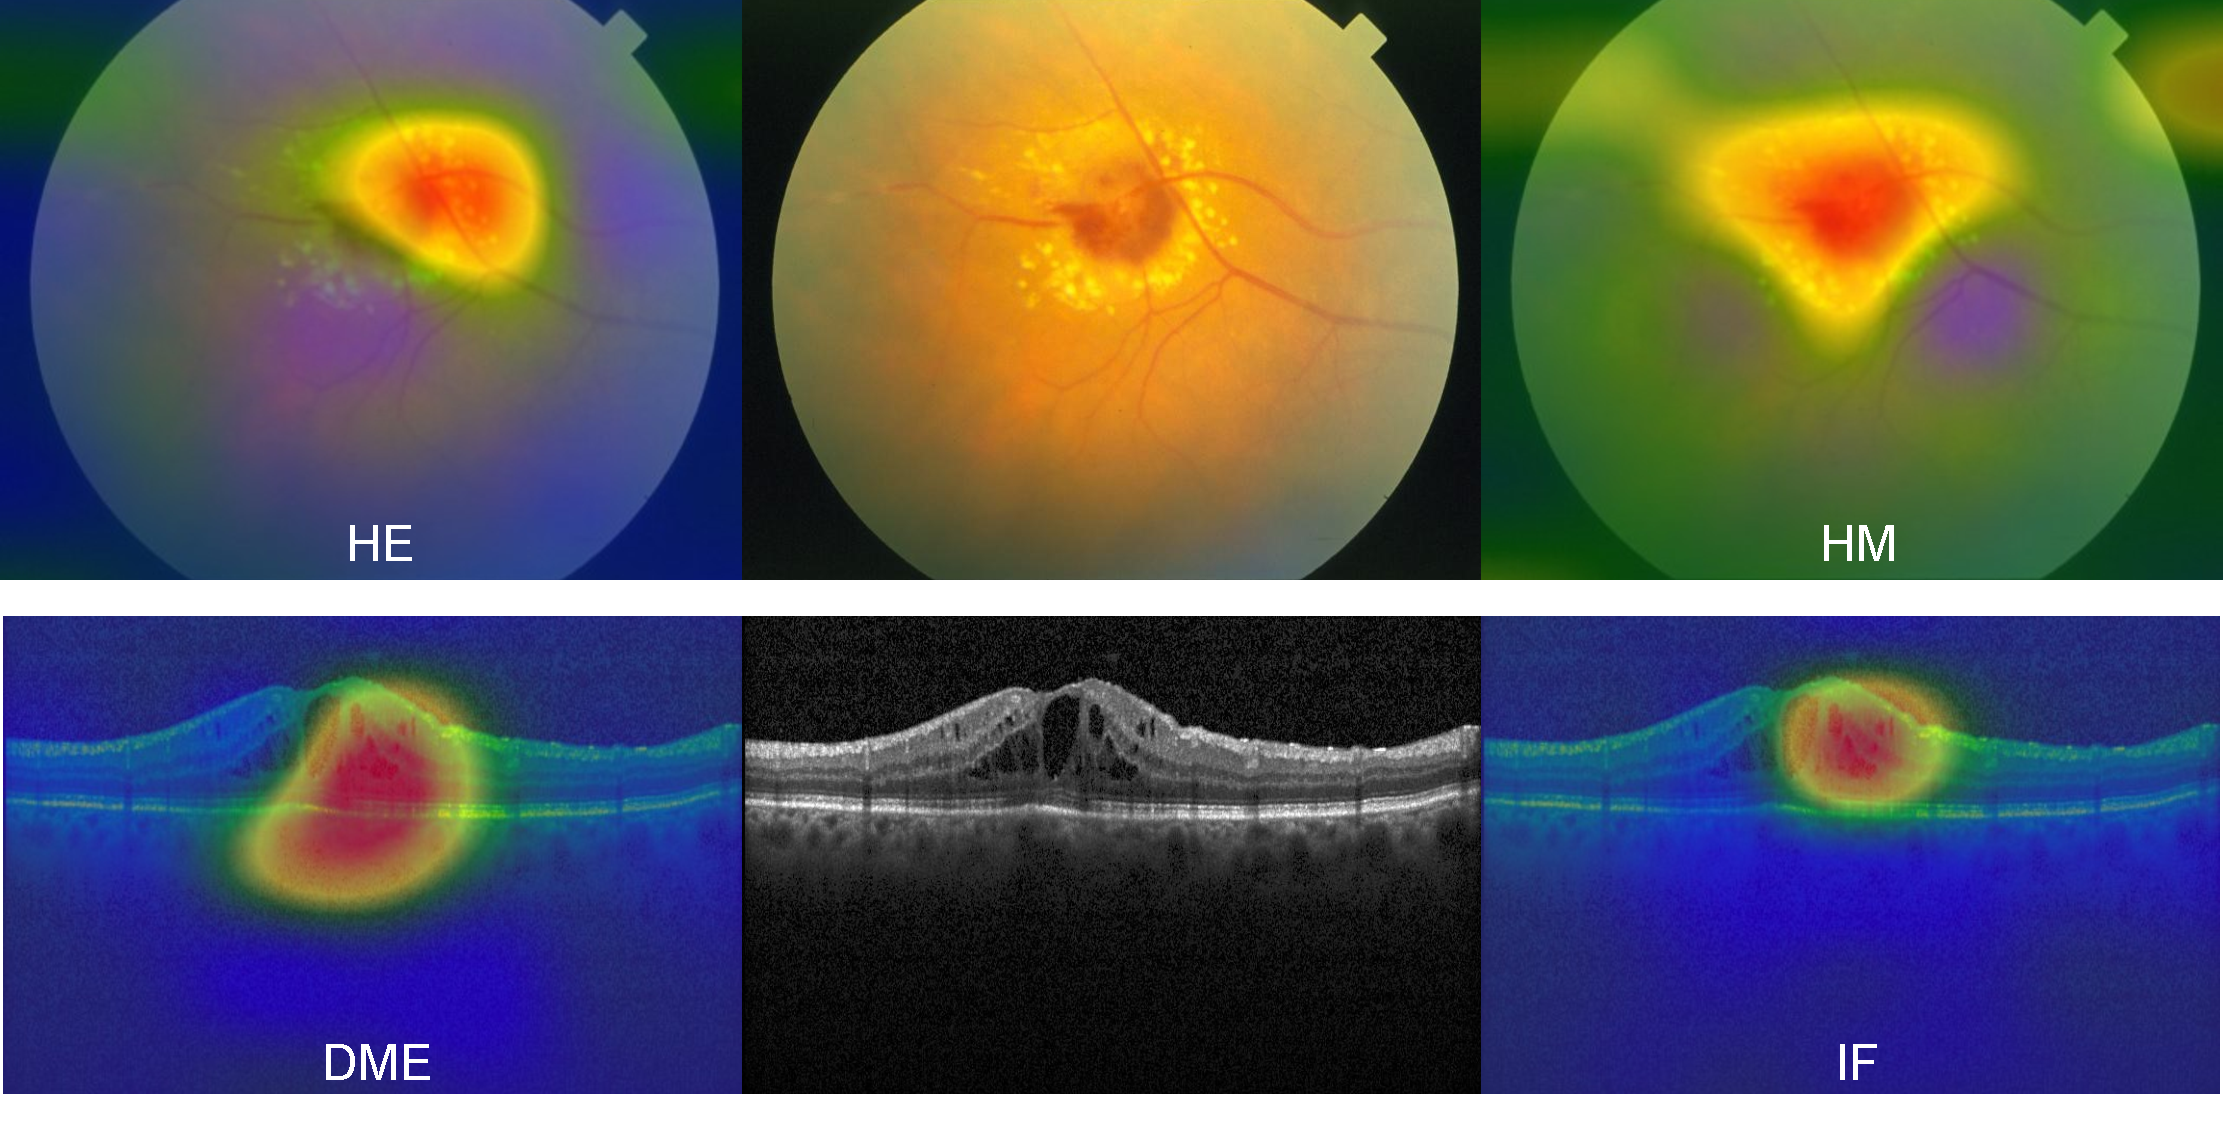
\includegraphics[width=0.8\linewidth]{Figs/abnormity_gradCAM_multiple_abnormities.pdf}
		\caption{GradCAM with multiple abnormities}
		\vspace{0.3cm}
		\label{fig:gradCAM_multi_abnormity}
	\end{figure}
	
	Fig.~\ref{fig:gradCAM_multi_abnormity} demonstrates that the Abnormity Models may be able to correctly identify multiple abnormities on an image. Knowing that OCT and fundus images often do include more than one abnormity, we employ a method to determine the codominant abnormities. We input an image to the Abnormity Models and get the abnormity probabilities vector. If the abnormity with the highest probability has probability greater than 0.9, it is regarded as dominant; if not, we continue taking the abnormity with the next high probability until either the sum of the probabilities of the chosen abnormities reaches 0.9, or the number of abnormities reaches the maximum, which is 4, and all the chosen abnormities are regarded as codominant. 
	
	This codominant abnormities method allows the Abnormity Models to identify multiple abnormities. For example, the fundus image in Fig.~\ref{fig:gradCAM_multi_abnormity} only has ground truth label ``HE'', but the Fundus Model correctly predicts that it has codominant abnormities ``HE'' and ``HM''. 
	
	\section{Diagnosis Model}
	
	\subsection{Data Preparation}
	
	In Stage D1, we prepare data 
	
	TEXT: how to choose data (with an example)
	how to find level (number of traits = level for the disease as label during training)
	
	
	\subsection{Training}
	
	%The model training is on a desktop computer with Intel$^®$ Xeon$^®$ Platinum 8352V Processor, 256GB of RAM and 2 NVIDIA GPU (GeForce RTX 4090) with 48GB VRAM. The training uses cross entropy loss, ADAM optimizer with learning rate 0.001, a batch size of 32 and five-fold cross-validation. The code is written with PyTorch in an Anaconda environment. Refer to ``Appendix'' for the link to the code repository on GitHub. 
	
	TEXT: comments
	
	
	\subsection{Results}
	
	TEXT: D1 output - calculate expected grade. in order to compare, divide by total number of traits for this disease so that normalized grade falls in [0, 1]. 
	used for checking number of abnormities associated to the disease
	
	TEXT: top-probs method
	
	\begin{table}[htbp]
		\centering
		\caption{Diagnosis Test}
		\label{tb:diagnosis_test}
		\pgfplotstabletypeset[
		multicolumn names,
		col sep=comma,
		columns = {Abnormity, Precision, Sensitivity, Specificity, FOne, AUC},
		columns/Abnormity/.style={string type, column name=Abnormities},
		columns/Precision/.style={string type, column name=Precision},
		columns/Sensitivity/.style={string type, column name=Sensitivity},
		columns/Specificity/.style={string type, column name=Specificity},
		columns/FOne/.style={string type, column name={F1 Score}},
		columns/AUC/.style={string type, column name=AUC},
		every head row/.style={before row=\toprule, after row=\midrule},
		every last row/.style={ after row=\bottomrule}
		]{Tables/diagnosis2.csv}
	\end{table}
	
	\begin{figure}[htbp]
		\centering
		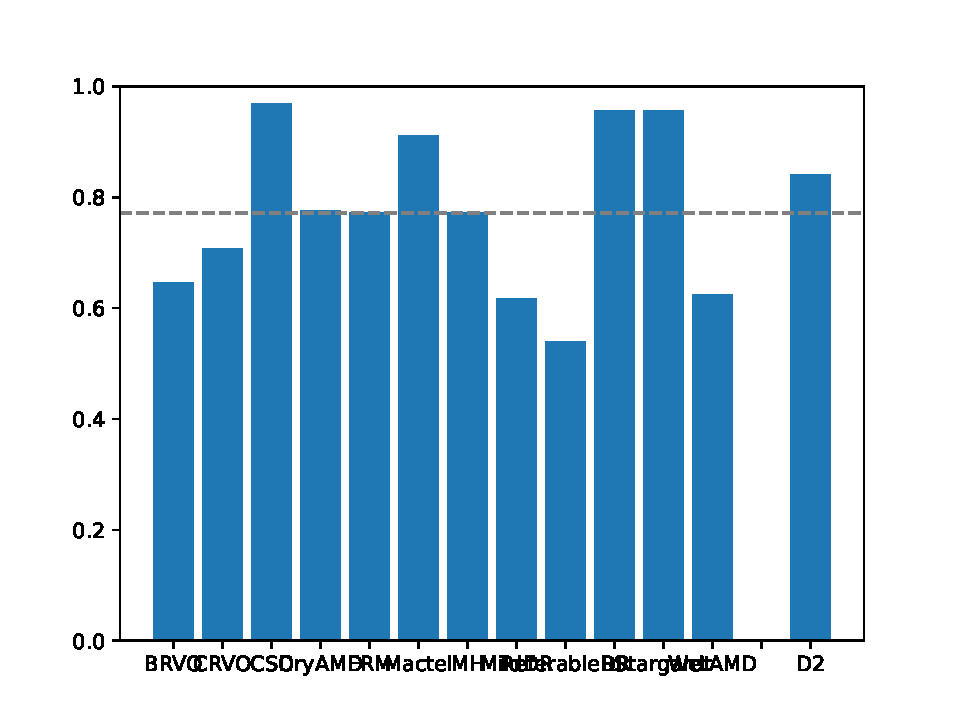
\includegraphics[width=\linewidth]{Figs/diagnosis1_acc_barchart.pdf}
		\caption{D1 Acc Bar}
		\vspace{0.3cm}
		\label{fig:D1_acc_bar}
	\end{figure}
	
	\begin{figure}[htbp]
		\centering
		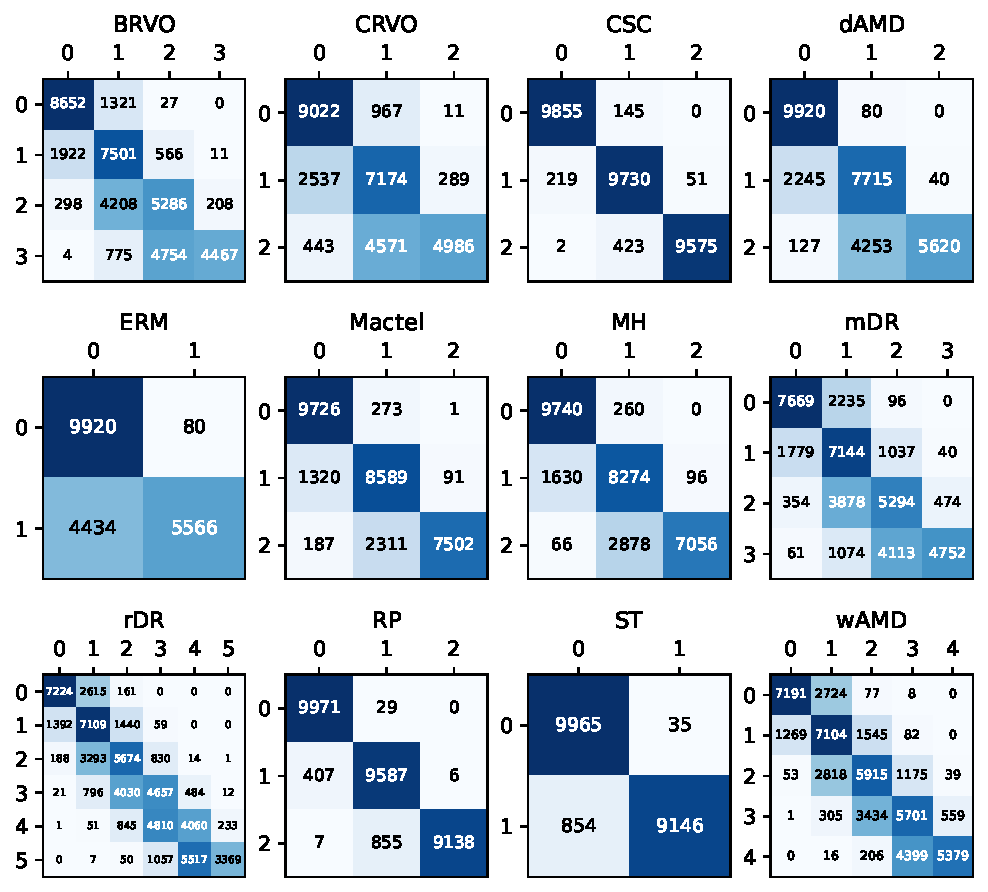
\includegraphics[width=\linewidth]{Figs/diagnosis1_confusion_matrix.pdf}
		\caption{D1 Conf Mat}
		\vspace{0.3cm}
		\label{fig:D1_conf_mat}
	\end{figure}
	TEXT: comments
	
	\begin{figure}[htbp]
		\centering
		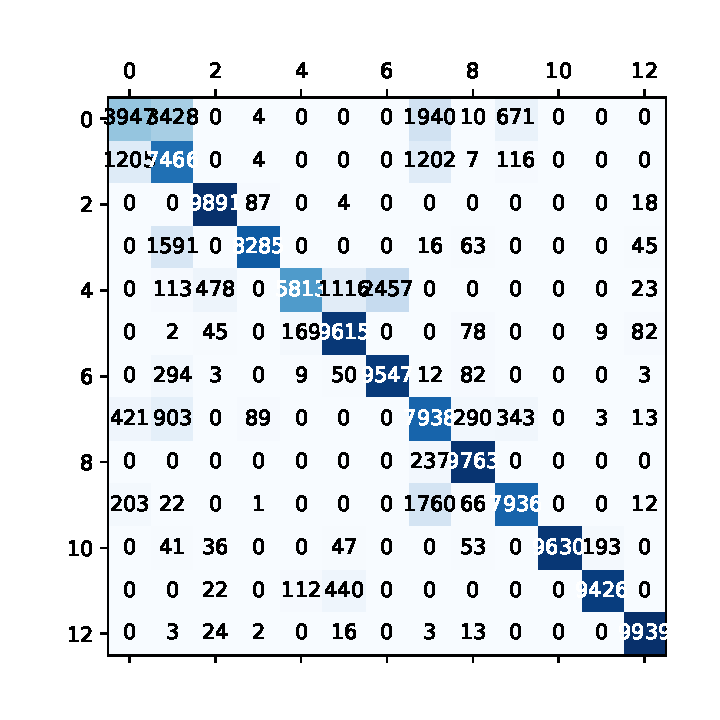
\includegraphics[width=\linewidth]{Figs/diagnosis2_confusion_matrix.pdf}
		\caption{D2 Conf Mat}
		\vspace{0.3cm}
		\label{fig:D2_conf_mat}
	\end{figure}
	\begin{figure}[htbp]
		\centering
		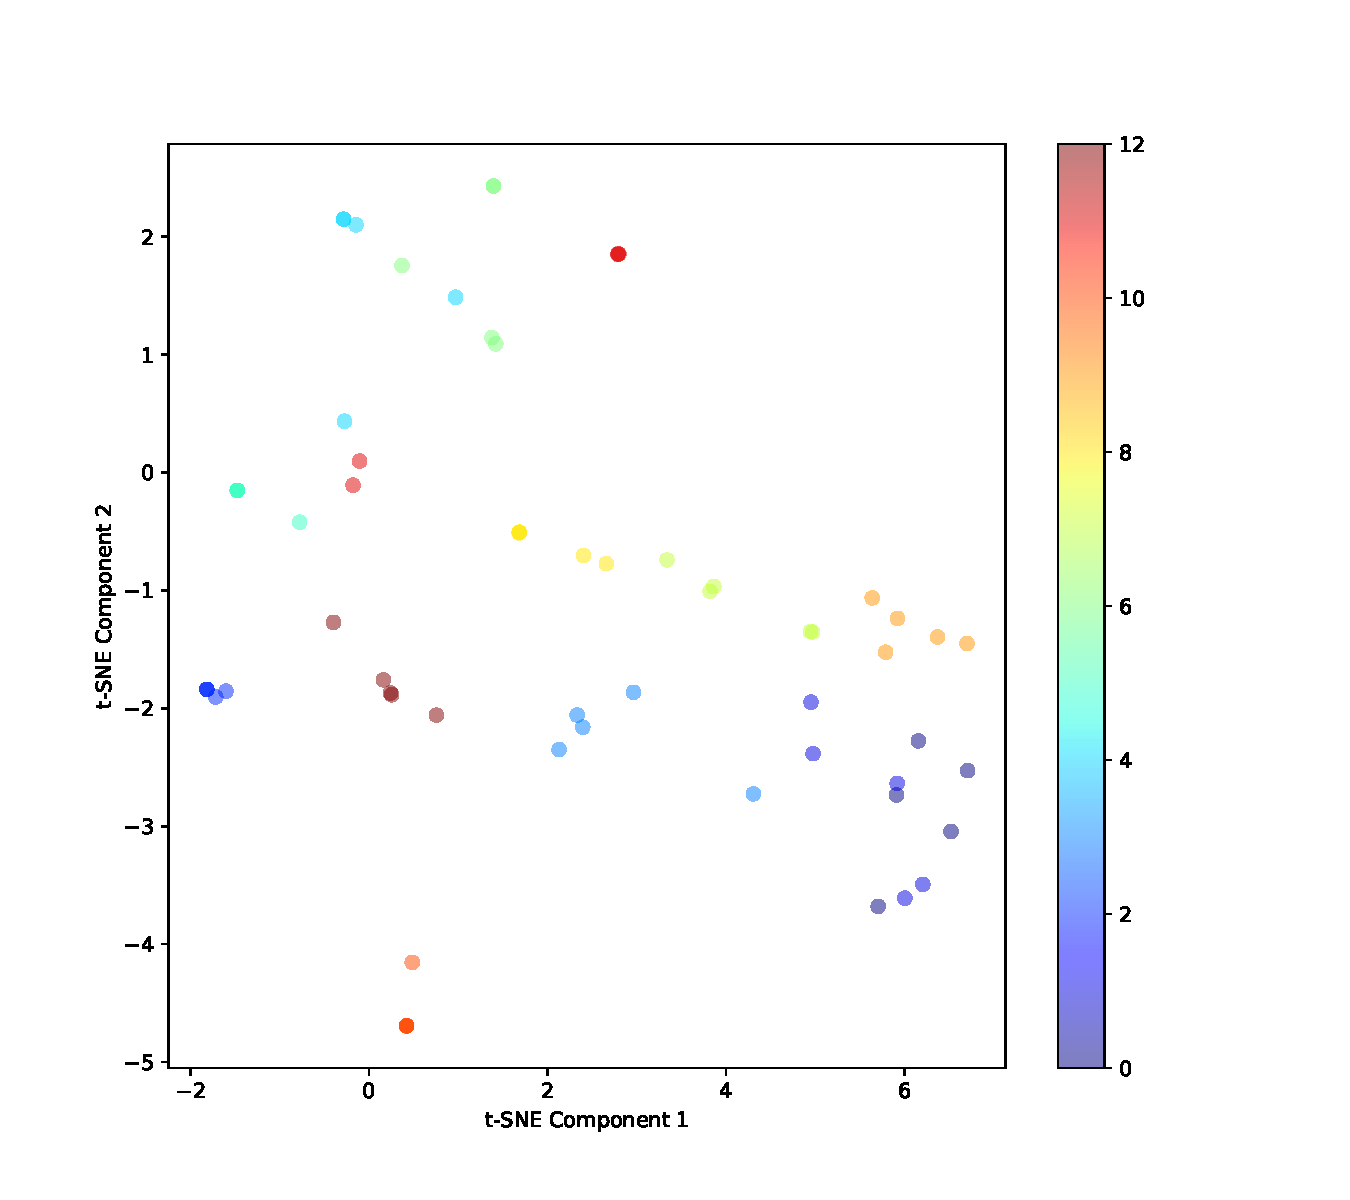
\includegraphics[width=\linewidth]{Figs/diagnosis2_tSNE.pdf}
		\caption{D2 tSNE}
		\vspace{0.3cm}
		\label{fig:D2_tSNE}
	\end{figure}
	TEXT: comments
	
	\begin{figure}[htbp]
		\centering
		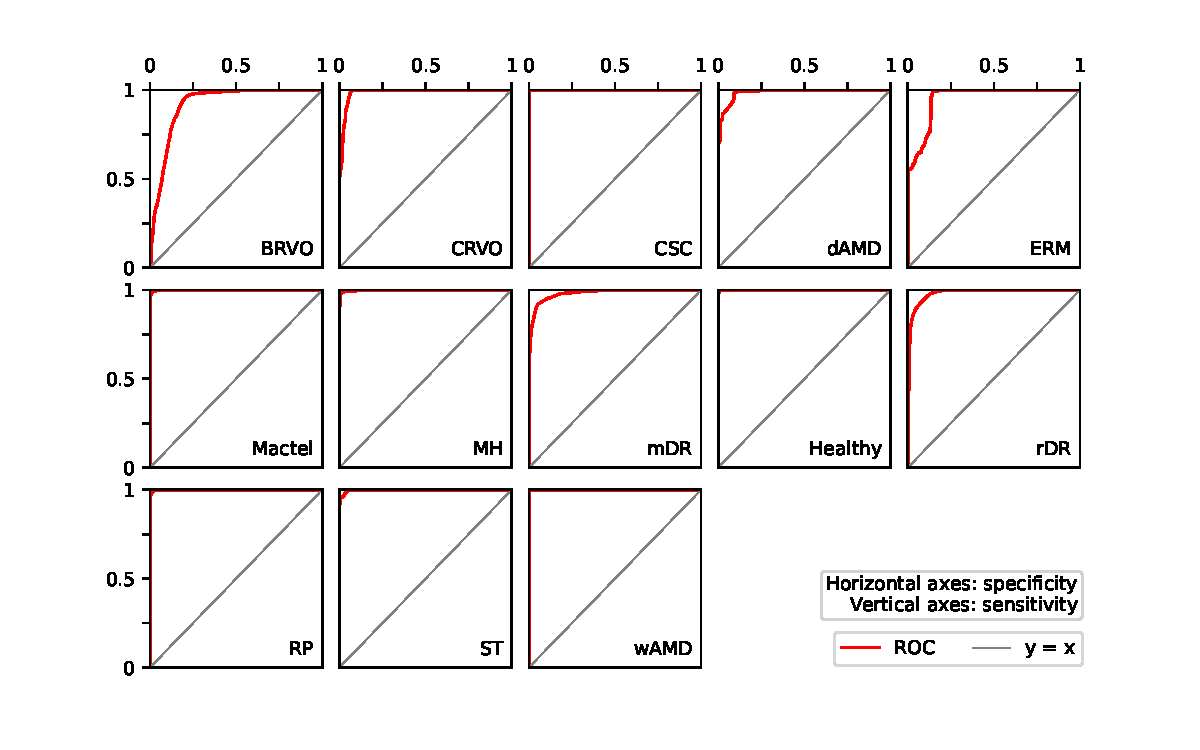
\includegraphics[width=\linewidth]{Figs/diagnosis2_ROC.pdf}
		\caption{D2 ROC}
		\vspace{0.3cm}
		\label{fig:D2_ROC}
	\end{figure}
	TEXT: comparison and comments
	
	\section{Discussion}
	
	TEXT: Do two models increase accuracy? How?
	
	TEXT: Comparison to other studies
	
	TEXT: Strengths and weaknesses
	how to improve
	
	\section{Conclusion}
	
	TEXT: conclusion
	
	\phantomsection
	\addcontentsline{toc}{section}{References}
	\newrefcontext[sorting=nyt]
	\printbibliography
	
	\pagebreak
	\section*{Appendix}
	
	List: Google Image source links
	
	Table: abnormities with description (edit the two tables below; ALPHABETICAL ORDER!!!)
	
	{
		\fontsize{9}{12}\selectfont
		{
			\begin{longtable}{lp{3.8in}}
				\caption{OCT Abnormities}
				\label{tb:oct-abnormites}\\
				\toprule
				Abnormity&Description\\
				\toprule
				
				\multicolumn{1}{l}{Central serous chorioretinopathy (CSC)}
				& \multicolumn{1}{l}{The accumulation of fluid underneath the retina.}\\
				
				\multicolumn{1}{l}{Epiretinal membrane (ERM)}
				& A thin layer of fibrous tissue forms on the surface of the retina, particularly the macula.\\
				
				\multicolumn{1}{l}{Macular hole (MH)}
				& Disruption or discontinuity in the normal retinal layers surrounding the macular hole.\\
				
				\multicolumn{1}{l}{Stargardt disease}
				& Thinning and atrophy of the retina. Disruption of photoreceptor layers. Presence of subretinal deposits.\\
				
				\multicolumn{1}{l}{Retinitis pigmentosa (RP)}
				& Thinning of the Retinal Layers. Disruption of Photoreceptor Layers. Attenuation of Retinal Vasculature.\\
				
				\multicolumn{1}{l}{Macular telangiectasia (Mactel)}
				& Abnormalities in the macular blood vessels, leading to changes in the macular structure and function\\
				
				\multicolumn{1}{l}{Diabetic macular edema (DME)}
				& The accumulation of fluid in the macula. \\
				
				\multicolumn{1}{l}{Choroidal neovascularization}
				& The abnormal growth of new blood vessels in the choroid layer.\\
				
				\multicolumn{1}{l}{Subretinal fluid}
				& The accumulation of fluid between the neurosensory retina and the retinal pigment epithelium (RPE)\\
				
				\multicolumn{1}{l}{Intraretinal fluid}
				& The accumulation of fluid within the layers of the retina.\\
				
				\multicolumn{1}{l}{Drusen}
				& Small deposits of extracellular material that accumulate beneath the retinal pigment epithelium (RPE) or between the RPE and the photoreceptor layer in the macular region of the retina.\\
				
				\bottomrule
			\end{longtable}
		}
	}
	
	{
		\fontsize{9}{12}\selectfont
		{
			\begin{longtable}{lp{3.8in}}
				\caption{Fundus Abnormalities}
				\label{tb:fundus-ab}\\
				\toprule
				Abnormity&Description\\
				\toprule
				
				\multicolumn{1}{l}{Retinitis pigmentosa (RP)}
				& Description of RP\\
				
				\multicolumn{1}{l}{Microaneurysm}
				& Description of microaneurysm\\
				
				\multicolumn{1}{l}{Macular hole (MH)} & Full-thickness macular hole showing a surrounding cuff of subretinal fluid.\\
				
				\multicolumn{1}{l}{Hard exudate} & Yellow or Yellow-White Deposits. Hard Borders. Distribution. Clustering Around Blood Vessels\\
				
				\multicolumn{1}{l}{Hemorrhage} & Small dot-like to larger blot. Fresh hemorrhages typically appear bright red or deep red in color, indicating the presence of oxygenated blood. Over time, as the blood undergoes degradation and clotting, the hemorrhage may change color to darker red, orange, or yellowish hues.\\
				
				\multicolumn{1}{l}{Cotton wool patch / soft exudate} & White or off-white lesions. Irregular shapes and margins.\\
				
				\multicolumn{1}{l}{Vascular abnormity} & Retinal Vessel Tortuosity. Retinal Vessel Caliber Changes. \\
				
				\multicolumn{1}{l}{Drusen} & Small, round or oval-shaped yellow or white deposits.\\
				
				\bottomrule
			\end{longtable}
		}
	}
	
	
	\begin{figure}[htbp]
		\centering
		
\includegraphics[width=\linewidth]{Figs/Temp.png}
		\caption{Result Page}
		\vspace{0.3cm}
		\label{fig:result_page}
	\end{figure}
	
	TEXT: APP/website description
	
	Link: GitHub repo
	
\end{document}